% ==============================================================================
% REVIEWER / FORMATTING NOTES:
% 
% 1. Fig. 1 (Trust Model): Simplified layout to a straight top-down flow.
%    Removed the "bend" angles from the arrows which caused overlapping text. 
%    The layout is now linear and much cleaner to read while retaining all 3 actors + platform.
% 2. Fig. 2 (Architecture): Significantly simplified the layout to a clean 3-tier vertical stack.
%    Removed the large bounding boxes (`fit`) that were blowing out the dimensions.
%    Ensured nodes are aligned in a standard grid (Client -> Compute/API -> Data).
%    Wrapped both in \resizebox{\columnwidth}{!} just in case, but they are natively much smaller now.
% 3. The rest of the document remains unchanged (Ablations, Security Analysis, Author Bio removed, etc.).
% ==============================================================================

\documentclass[journal,twoside,10pt]{IEEEtran}

% ─── Packages ─────────────────────────────────────────────────────────────────
\usepackage[T1]{fontenc}
\usepackage[utf8]{inputenc}
\usepackage{amsmath,amssymb,amsfonts}
\usepackage{algorithmic}
\usepackage{graphicx}
\usepackage{textcomp}
\usepackage{xcolor}
\usepackage{booktabs}
\usepackage{multirow}
\usepackage{array}
\usepackage{url}
\usepackage{hyperref}
\usepackage{tikz}
\usepackage{pgfplots}
\pgfplotsset{compat=1.18}
\usetikzlibrary{shapes.geometric, arrows.meta, positioning, fit, backgrounds,
                decorations.pathreplacing, calc, matrix, chains}

% ─── TikZ styles ──────────────────────────────────────────────────────────────
\tikzset{
  block/.style={rectangle, draw=black!70, fill=blue!8, rounded corners=3pt,
                minimum width=2.4cm, minimum height=0.8cm, text width=2.2cm,
                align=center, font=\scriptsize, line width=0.5pt},
  actor/.style={rectangle, draw=black!80, fill=gray!12, rounded corners=4pt,
                minimum width=2.6cm, minimum height=0.8cm, text width=2.4cm,
                align=center, font=\scriptsize\bfseries, line width=0.7pt},
  process/.style={rectangle, draw=black!70, fill=green!8, rounded corners=3pt,
                  minimum width=2.8cm, minimum height=0.8cm, text width=2.6cm,
                  align=center, font=\scriptsize, line width=0.5pt},
  storage/.style={cylinder, draw=black!70, fill=yellow!10, shape border rotate=90,
                  minimum width=1.6cm, minimum height=0.7cm, text centered,
                  font=\scriptsize, line width=0.5pt},
  arrow/.style={-{Stealth[length=4pt]}, draw=black!70, line width=0.6pt},
  darrow/.style={<->, draw=black!60, line width=0.5pt, dashed},
  label/.style={font=\scriptsize, text=black!80, fill=white, inner sep=1pt},
}

% ─── Hyperref ─────────────────────────────────────────────────────────────────
\hypersetup{colorlinks=true, linkcolor=blue!60!black, citecolor=green!40!black,
            urlcolor=blue!60!black}

\begin{document}

\title{ZK-Auth: A Zero-Knowledge Proof-Based Authentication\\
Framework with Selective Disclosure and\\
Continuous Behavioral Biometric Verification}

\author{Abhay~Dandge\IEEEmembership{}\\
  Department of Computer Science and Engineering,\\
  Maulana Azad National Institute of Technology, Bhopal, India\\
  \textit{Email: abhay.dandge@manit.ac.in}
}

\markboth{IEEE TRANSACTIONS ON INFORMATION FORENSICS AND SECURITY}{}

\maketitle

% ─── ABSTRACT ─────────────────────────────────────────────────────────────────
\begin{abstract}
Contemporary authentication systems suffer from a fundamental tension: they
require users to disclose personal information to verify identity, creating
privacy exposure proportional to access frequency. This paper presents
\textsc{ZK-Auth}, a cryptographic authentication infrastructure that resolves
this tension through three integrated mechanisms, implemented as an
\textbf{OAuth 2.0 Authorization Server in which the conventional
password-based login step of the Authorization Code grant is replaced by a
zero-knowledge proof} --- the same architectural pattern underlying
``Sign in with Apple,'' which pairs OAuth/OIDC delegation with a
non-password authenticator. First, we replace the password-login step with
Groth16 zero-knowledge succinct non-interactive arguments of knowledge
(zk-SNARKs) over the BN254 elliptic curve, enabling users to prove knowledge
of a registration secret without transmitting it; the resulting proof
authorizes a short-lived OAuth authorization code rather than a
password-backed session token. Second, we implement selective credential
disclosure via Poseidon hash-based Merkle trees, allowing holders to prove
individual attribute predicates (e.g., $\text{age} \geq 18$) without
exposing remaining attributes or raw values. Third, we address the
session-continuity gap inherent in one-time authentication proofs through an
LSTM-based behavioral biometric monitor that computes continuous risk scores
from six telemetry features, triggering cryptographic step-up
re-authentication on anomaly detection. The system is architected around W3C
Decentralized Identifiers (DIDs) and Verifiable Credentials (VCs) in a
three-actor trust model---Issuer, Holder, Verifier---with per-institution
Ed25519 signing keys held exclusively by registered issuers. We evaluate
ZK-Auth across four heterogeneous deployment environments: a Node.js server
(Apple M4), a Chrome browser client (Web Worker WASM), and two Android
mobile devices spanning a flagship-to-midrange hardware spread (Samsung
Galaxy S23 and Galaxy Tab~S9 FE+). Across $n=120$ consecutive server-side
trials, ZK-Auth achieves a median end-to-end login latency of 132.5\,ms
(100\% success rate)---23\% faster than the Argon2id hashing step alone in
a comparable password-based system (172.8\,ms median)---with a compact
Groth16 proof size of $\sim$723\,bytes. Client-side proof generation ranges
from 62\,ms (Node.js) to 361\,ms (mid-tier Android tablet), and the LSTM
behavioral model, trained on the public Balabit Mouse Dynamics dataset
(108{,}111 windows), achieves AUC-ROC 0.816 with a 6.15\% false-accept rate.
We further provide formal security proofs for soundness, zero-knowledge,
and nullifier replay resistance, a quantitative comparison against seven
existing authentication paradigms---including pure OAuth~2.0/OIDC without a
ZKP-backed authenticator---and a scalability analysis showing $K$-linear
horizontal throughput scaling compatible with national-identity-scale
deployments such as India's DigiLocker (434.9~million users). These results
establish that pairing OAuth~2.0 delegation with a ZKP-based authentication
primitive is not merely privacy-preserving in theory but practically
deployable at production latency across the full range of client hardware,
with direct implications for cloud security, decentralized identity, and
regulatory compliance under India's DPDP Act 2023 and the EU GDPR.
\end{abstract}

\begin{IEEEkeywords}
behavioral biometrics, BN254 elliptic curve, continuous authentication,
decentralized identity, Groth16 zk-SNARK, LSTM neural networks, Merkle trees,
OAuth 2.0 Authorization Code grant, Poseidon hash function, selective
disclosure, session security, verifiable credentials, W3C DID,
zero-knowledge proofs
\end{IEEEkeywords}

% ═══════════════════════════════════════════════════════════════════════════════
\section{Introduction}
% ═══════════════════════════════════════════════════════════════════════════════

\IEEEPARstart{T}{he} proliferation of digital services has made authentication
a central security concern. Password-based authentication---despite decades of
documented weaknesses including credential stuffing, phishing, and database
breaches---remains the dominant paradigm. Industry breach reports consistently
attribute the plurality of confirmed data breaches to credential-based attack
vectors~\cite{dbir}, and the average cost of a credential-stuffing-related breach has
risen year over year as attackers automate large-scale leaked-password reuse
against unrelated services. Even modern alternatives such as OAuth~2.0 and
SAML~\cite{saml} delegate trust to centralized identity providers, preserving the
fundamental weakness: the authenticating party must be trusted with user
credentials or session tokens, and a single provider compromise exposes all
dependent services. Passkeys and WebAuthn/FIDO2~\cite{fido2} eliminate
shared-secret transmission but still bind authentication to a specific
device-bound credential without offering attribute-level selective
disclosure or built-in session-continuity monitoring.

Zero-knowledge proofs (ZKPs) provide a cryptographically sound solution:
A prover can demonstrate to a verifier the validity of a statement without
disclosing anything more than the statement~\cite{gmr89}. When used for
authentication, a user can prove possession of a registration secret using
a ZKP without disclosing the secret itself---thereby addressing the key
weakness of credential theft, database breaches, and offline attacks
against stored hashes. Yet, there are four issues associated with use of
ZKPs for authentication in production systems that have been studied
independently but not together.

\textit{Challenge 1 (Proof complexity and cross-environment latency):} Generation of proof
is a computationally complex task and needs an efficient circuit design
and implementation on the client side, keeping latency acceptable for
users---not just developers’ workstations but also diverse client
hardware including desktops, premium phones, and mid-range tablets.

\textit{Challenge 2 (Attribute-level privacy):} True practical use cases would need demonstrating certain characteristics about an identity (age, nationality, affiliation with an institution) selectively---an ability which standard ZKP authentication does not offer.

\textit{Challenge 3 (Session continuity):} One-time authentication proofs
cannot protect against session hijacking after initial proof acceptance;
a separate mechanism is required for continuous identity assurance that does
not itself become a new authentication bottleneck or false-rejection source.

\textit{Challenge 4 (Verifiable empirical grounding):} Much of the published
literature on ZKP authentication reports proof-generation benchmarks from a
single environment (typically a development workstation), leaving open the
question of whether the approach is viable across the actual deployment
surface of a consumer-facing system.

\textit{Challenge 5 (Relying-party delegation compatibility):} Much prior
ZKP-authentication work implicitly treats ZKP as a replacement for the
entire authentication and authorization stack, rather than as a primitive
that can be substituted underneath an existing delegation protocol such as
OAuth~2.0. This creates a deployment barrier: an institution with existing
OAuth-based relying-party integrations cannot adopt ZKP authentication
without discarding that integration surface. We address this by
implementing ZK-Auth \textit{as} an OAuth~2.0 Authorization Server, with
the ZKP substituting only for the conventional password-login step.

This paper makes the following contributions:

\begin{enumerate}
  \item We design and implement \textsc{ZK-Auth}, a complete authentication
        infrastructure using Groth16 zk-SNARKs over BN254 with a
        Circom-compiled circuit of \textbf{932 constraints and 935 wires}
        (verified via \texttt{snarkjs r1cs info}), deployed for both
        server-side and client-side WebAssembly execution, and wrapped in
        a working \textbf{OAuth~2.0 Authorization Code flow with PKCE}
        so the proof substitutes for the conventional password-login step
        rather than for OAuth's relying-party delegation layer entirely.

  \item We implement selective credential disclosure via a depth-8 Poseidon
        Merkle tree commitment scheme compatible with the W3C Verifiable
        Credentials standard, enabling per-attribute GTE/LTE/EQ predicate
        proofs without revealing attribute values to verifiers.

  \item We address the session-continuity gap through an LSTM behavioral
        biometric model operating on a 50-event sliding window of six
        telemetry features, with EMA-smoothed risk scoring and automated
        step-up re-authentication, trained and evaluated on a public
        behavioral biometrics dataset rather than synthetic data.

  \item We design a multi-tenant credential issuance infrastructure with
        per-institution Ed25519 keypair generation and W3C DID publication,
        implementing a PKI-analogous root-of-trust model.

  \item We provide a formal security analysis covering soundness,
        zero-knowledge, nullifier replay prevention, Merkle commitment
        collision resistance, OAuth authorization-code binding, and
        adversarial behavioral model robustness, together with an
        explicit threat model and attacker capability enumeration.

  \item We report empirical measurements of ZK-Auth end-to-end login latency
        across \textbf{four distinct execution environments}---Node.js
        server, Chrome browser (Web Worker WASM), and two Android devices
        spanning flagship-to-midrange hardware---against an Argon2id
        baseline, demonstrating that ZKP authentication is measurably
        competitive with the dominant cost of password-based authentication
        across the realistic deployment surface.

  \item We quantify server-side horizontal scalability under concurrent
        load and derive deployment sizing guidance for national-identity-
        scale systems such as India's DigiLocker, and present a
        quantitative and qualitative baseline comparison against seven
        existing authentication paradigms.
\end{enumerate}

The remainder of this paper is organized as follows.
Section~\ref{sec:related} reviews related work.
Section~\ref{sec:architecture} presents the architecture, threat model, and
the system's relationship to OAuth~2.0.
Section~\ref{sec:zkp} details the ZKP protocol and circuit.
Section~\ref{sec:disclosure} describes selective disclosure.
Section~\ref{sec:behavioral} presents the behavioral biometric subsystem.
Section~\ref{sec:issuer} covers multi-tenant issuance.
Section~\ref{sec:security} provides security analysis.
Section~\ref{sec:results} presents experimental results.
Section~\ref{sec:discussion} discusses deployment implications.
Section~\ref{sec:conclusion} concludes.

% ═══════════════════════════════════════════════════════════════════════════════
\section{Literature Survey}
\label{sec:related}
% ═══════════════════════════════════════════════════════════════════════════════

\subsection{Zero-Knowledge Proof Systems}

The theoretical foundations of zero-knowledge proofs were established by
Goldwasser, Micali, and Rackoff~\cite{gmr89}, with subsequent work on
non-interactive proofs by Blum, Feldman, and Micali~\cite{bfm88} and the
Fiat--Shamir heuristic for transforming interactive proofs into
non-interactive ones~\cite{fiatshamir}. Practical zk-SNARK systems became
feasible with Pinocchio~\cite{parno13} and the quadratic arithmetic program
(QAP) formulation of Gennaro et al.~\cite{gennaro13}, and were significantly
improved by Groth16~\cite{groth16}, which achieves constant-size proofs
(three group elements) with $\mathcal{O}(1)$ pairing verifications. Bitansky et al.~\cite{bitansky12} formalized the extractable
knowledge assumptions underlying succinct argument soundness.

Groth16 has been widely deployed in blockchain contexts; Zcash~\cite{zcash14}
uses it for shielded transactions with $\sim$2 second proof generation on
desktop hardware. PLONK~\cite{plonk}
and Halo2~\cite{halo2} eliminate the circuit-specific trusted setup at the
cost of larger proofs and higher verification time; STARKs~\cite{starks}
remove trusted setup entirely via FRI-based polynomial commitments but incur
proof sizes an order of magnitude larger than Groth16. Bulletproofs~\cite{bulletproofs}
target range proofs without trusted setup. For our authentication context---a
small, fixed circuit requiring short proofs and fast server-side
verification at high request volume---Groth16's circuit-specific trusted
setup is an acceptable cost in exchange for the smallest available proof
size and fastest verification.

\subsection{ZKP-Based Authentication}

ZKlogin~\cite{zklogin} applies ZKPs to OAuth-based Web3 authentication using
a centralized JWT oracle, inheriting OAuth's trust assumptions.
Semaphore~\cite{semaphore} implements anonymous group membership signaling
suitable for whistleblowing and voting applications but does not address
individual authentication, session management, or selective attribute
disclosure. SpartanNIZK~\cite{spartan} and Nova~\cite{nova} propose efficient
NIZK and incrementally-verifiable-computation systems without trusted setup.
Anonymous credential systems built on idemix~\cite{idemix} predate modern
SNARK tooling and rely on RSA-based commitments. Our work differs from all of the above by
targeting the complete authentication lifecycle---registration, login,
session continuity, and attribute-selective verification---within a single
standard web/mobile deployment.

\subsection{Selective Disclosure Credentials}

Selective disclosure has been addressed through BBS+ signatures~\cite{bbs},
which support message-level disclosure with multi-message signing and have
been standardized for verifiable credentials via the BBS+ IETF
draft~\cite{bbsplus}. The W3C Verifiable Credentials Data Model~\cite{w3cvc}
provides the structural framework for credential representation that
ZK-Auth's issuance layer adheres to. SD-JWT~\cite{sdjwt} offers a practical
but non-ZK approach where verifiers still receive selected attribute values
directly in cleartext. Anonymous credentials via CL signatures~\cite{cl} provide
ZK-based selective disclosure but require trusted setup per issuer. Mercurial
signatures~\cite{mercurial} extend delegatable anonymous credentials. Our Poseidon Merkle approach provides strictly stronger privacy than
SD-JWT: verifiers receive only boolean predicate results with no attribute
value exposure, even for ``proved'' attributes.

\subsection{Behavioral Biometrics for Continuous Authentication}

Continuous authentication via behavioral biometrics has been studied using
keystroke dynamics~\cite{shepherd95,monrose00}, mouse movement
patterns~\cite{nakkabi11,ahmed07}, and touch gestures~\cite{frank13}. Deep
learning approaches---particularly recurrent architectures---have
demonstrated strong performance on temporal behavioral sequences. TypeNet~\cite{typenet}
applies LSTM-based keystroke analysis achieving $>$98\% genuine acceptance
on free-text typing; Acien et al.~\cite{acien21} extend this with
attention-based sequence models.
BehaveFormer~\cite{behaveformer} applies transformer architectures to
combined touch-and-keystroke streams.
TypingDNA~\cite{typingdna} deploys keystroke biometrics commercially, and BioCatch~\cite{biocatch} offers a commercial behavioral
fraud-detection platform. Our
contribution integrates behavioral monitoring as a \textit{post-ZKP
session-continuity layer} with cryptographic step-up re-authentication.

\subsection{Decentralized Identity}

The W3C DID specification~\cite{w3cdid} provides a standards-based framework
for decentralized identifiers independent of centralized registries. The
Self-Sovereign Identity (SSI) movement~\cite{allen16} has produced
implementations including Hyperledger Indy~\cite{hyperledgerindy}, IOTA
Identity, and Microsoft ION. Sovrin~\cite{sovrin} provides a
public-permissioned ledger purpose-built for SSI credential revocation
registries. ZK-Auth
integrates DID-anchored credential issuance with ZKP-based authentication
within a single deployable system.

\subsection{Authentication and Behavioral Datasets}

Public benchmark datasets are essential for reproducible behavioral
biometrics research. The Balabit Mouse Dynamics Challenge~\cite{balabit}
used in this work provides labeled genuine/intruder mouse-event sessions
across ten users. The CMU keystroke dataset~\cite{killourhy09} offers a
comparable benchmark for keystroke timing but was not used here since
ZK-Auth's current telemetry pipeline targets mouse-dominant desktop
interaction.

% ═══════════════════════════════════════════════════════════════════════════════
\section{Proposed System Architecture}
\label{sec:architecture}
% ═══════════════════════════════════════════════════════════════════════════════

\subsection{Threat Model}

We consider an adversary $\mathcal{A}$ with the following capabilities:
(i)~passive observation of all client--server communications;
(ii)~active modification of server-side database records excluding key
material protected by the platform's key-management boundary;
(iii)~compromise of a subset of verifier nodes;
(iv)~knowledge of the circuit structure, verification keys, and commitment
values;
(v)~access to behavioral telemetry from other users for model inference.

We explicitly exclude cryptographic breaks of the BN254 discrete logarithm
problem, Poseidon hash preimage resistance, or Ed25519 signature forgery.

Security goals: (G1)~authentication soundness; (G2)~zero-knowledge during
proof; (G3)~nullifier replay prevention; (G4)~selective disclosure privacy; (G5)~session-continuity
assurance.

\subsection{Three-Actor Trust Model}

\textsc{ZK-Auth} implements the W3C Verifiable Credentials trust triangle
with three actors as illustrated in Fig.~\ref{fig:trust_model}.

\begin{figure}[!t]
\centering
\resizebox{0.85\columnwidth}{!}{%
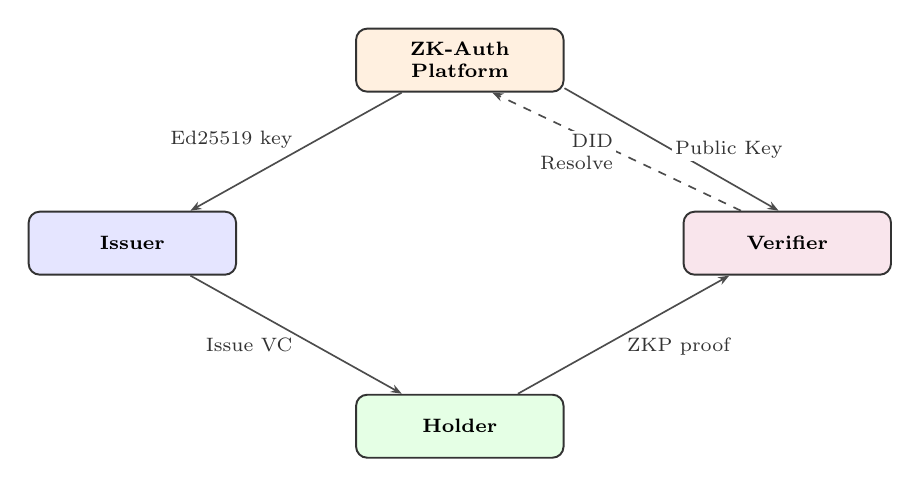
\begin{tikzpicture}[node distance=1.5cm and 1.5cm]
  % Nodes
  \node[actor, fill=orange!12] (platform) {ZK-Auth Platform};
  \node[actor, fill=blue!10, below left=of platform] (issuer) {Issuer};
  \node[actor, fill=purple!10, below right=of platform] (verifier) {Verifier};
  \node[actor, fill=green!10, below right=of issuer] (holder) {Holder};

  % Edges (Straight, simple arrows using specific anchor points to prevent overlap)
  \draw[arrow] (platform) -- node[label, above left] {Ed25519 key} (issuer);
  \draw[arrow] (issuer) -- node[label, below left] {Issue VC} (holder);
  \draw[arrow] (holder) -- node[label, below right] {ZKP proof} (verifier);
  
  % Shifted anchors for Verifier <-> Platform to keep lines straight but separated
  \draw[arrow, dashed] (verifier.145) -- node[label, left, align=right] {DID\\Resolve} (platform.315);
  \draw[arrow] (platform.345) -- node[label, right] {Public Key} (verifier.105);

\end{tikzpicture}%
}
\caption{Three-actor trust model. The ZK-Auth Platform acts as the root authority, authorizing institutions (Issuers) with unique keypairs. Holders receive credentials and submit proofs to Verifiers.}
\label{fig:trust_model}
\end{figure}


\begin{figure}[!t]
\centering
\resizebox{0.85\columnwidth}{!}{%
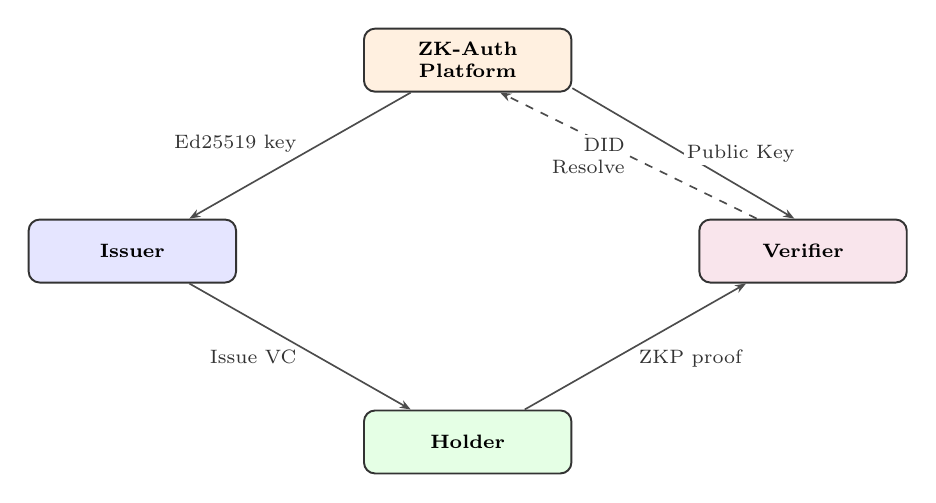
\begin{tikzpicture}[node distance=1.6cm and 1.6cm]
  % Nodes
  \node[actor, fill=orange!12] (platform) {ZK-Auth Platform};
  \node[actor, fill=blue!10, below left=of platform] (issuer) {Issuer};
  \node[actor, fill=purple!10, below right=of platform] (verifier) {Verifier};
  \node[actor, fill=green!10, below right=of issuer] (holder) {Holder};

  % Edges (Straight arrows with offset anchors to prevent bidirectional overlap)
  \draw[arrow] (platform) -- node[label, above left] {Ed25519 key} (issuer);
  \draw[arrow] (issuer) -- node[label, below left] {Issue VC} (holder);
  \draw[arrow] (holder) -- node[label, below right] {ZKP proof} (verifier);
  
  % Offset anchors (145/315 and 345/105 degrees) keep these two lines parallel but separated
  \draw[arrow, dashed] (verifier.145) -- node[label, left, align=right] {DID\\Resolve} (platform.315);
  \draw[arrow] (platform.345) -- node[label, right] {Public Key} (verifier.105);

\end{tikzpicture}%
}
\caption{Three-actor trust model. The ZK-Auth Platform acts as the root authority, authorizing institutions (Issuers) with unique keypairs. Holders receive credentials and submit proofs to Verifiers.}
\label{fig:trust_model}
\end{figure}


\begin{figure}[!t]
\centering
\resizebox{0.95\columnwidth}{!}{%
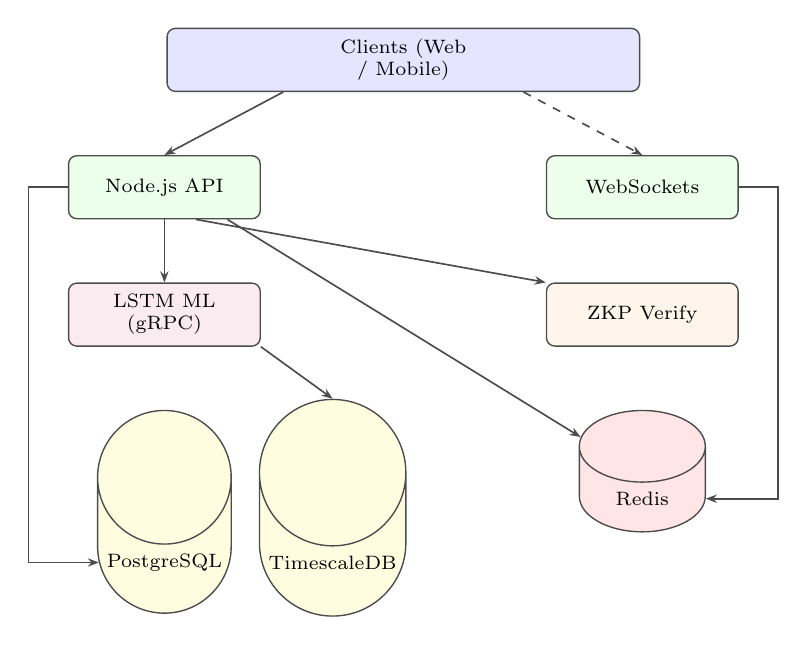
\begin{tikzpicture}[node distance=0.8cm and 0.4cm]
  % Client
  \node[block, fill=blue!10, minimum width=6cm] (clients) {Clients (Web / Mobile)};
  
  % API/Gateway layer
  \node[block, fill=green!8, below left=0.8cm and -1.2cm of clients] (api) {Node.js API};
  \node[block, fill=green!8, below right=0.8cm and -1.2cm of clients] (ws) {WebSockets};
  
  % Compute Layer
  \node[block, fill=purple!8, below=of api] (ml) {LSTM ML (gRPC)};
  \node[block, fill=orange!8, below=of ws] (zkp) {ZKP Verify};
  
  % Storage Layer
  \node[storage, fill=yellow!12, below=0.8cm of ml] (pg) {PostgreSQL};
  \node[storage, fill=yellow!12, right=0.4cm of pg] (ts) {TimescaleDB};
  \node[storage, fill=red!10, below=0.8cm of zkp] (redis) {Redis};
  
  % Edges
  \draw[arrow] (clients.195) -- (api.north);
  \draw[arrow, dashed] (clients.345) -- (ws.north);
  
  % API down to Compute/Storage (using shifted anchors on API's bottom edge to prevent crossing)
  \draw[arrow] (api.south) -- (ml.north);
  \draw[arrow] ([xshift=0.4cm]api.south) -- (zkp.north west);
  \draw[arrow] ([xshift=0.8cm]api.south) -- (redis.north west);
  
  % Route API to PG by going out the left side and down (bypasses ML block)
  \draw[arrow] (api.west) -- ++(-0.5,0) |- (pg.west);
  
  % ML to TS
  \draw[arrow] (ml.south east) -- (ts.north);
  
  % Route WS to Redis by going out the right side and down (bypasses ZKP block)
  \draw[arrow] (ws.east) -- ++(0.5,0) |- (redis.east);

\end{tikzpicture}%
}
\caption{ZK-Auth system component architecture. Clients interface with the Node.js API (REST) and WebSockets. The compute tier handles ML risk scoring and ZKP verification. Data is persisted in PostgreSQL, while Redis manages ephemeral session nonces.}
\label{fig:system_overview}
\end{figure}
}
\caption{System Component Architecture. Clients interface with the Node.js API (REST) and WebSockets. The compute tier handles ML risk scoring and ZKP verification. Data is persisted in PostgreSQL, while Redis manages ephemeral session nonces.}
\label{fig:system_overview}
\end{figure}

\textbf{Issuer:} An institution that is registered using a unique Ed25519 key-pair and a DID. The issuer performs Poseidon Merkle commitments, issues W3C VCs and saves only the Merkle root---never the actual attributes.

\textbf{Holder:} A person having a ZK wallet containing the 32-byte registration secret, the issued VC and a BIP-39 mnemonic. Proof generation happens locally (WASM on browser; WebView/JS on mobile).

\textbf{Verifier:} A relying party that publishes a proof request, receives
a ZKP-verified Verifiable Presentation, resolves the issuer DID, and records
only boolean predicate results.

\subsection{ZK-Auth as an OAuth 2.0 Authorization Server}
\label{sec:oauth_zkp}

ZK-Auth is, structurally, an \textbf{OAuth~2.0 Authorization Server
implementing the RFC~6749~\cite{oauth2} Authorization Code grant}, in
which the conventional ``user authenticates with a password'' step of
that grant is replaced with the Groth16 challenge/verify exchange
described in Section~\ref{sec:zkp}. ZKP and OAuth are not competing
designs; they operate at two different layers of the same protocol
stack. The OAuth layer governs \textit{which} relying party is
requesting access, \textit{what} scope it is requesting, \textit{where}
the user is redirected afterward, and how a short-lived authorization
code is exchanged for an access token---exactly the role OAuth plays in
any conventional deployment. The ZKP layer governs \textit{how} the
user proves identity within that delegation contract: ZK-Auth
substitutes a Groth16 proof of knowledge of the registration secret $s$
for the password-and-session-cookie check a conventional OAuth
Authorization Server would otherwise perform at this step. This is
structurally identical to ``Sign in with Apple'' and other federated-login
systems that pair OAuth/OIDC with a biometric authenticator (Face~ID,
Touch~ID) instead of a password---OAuth has always treated the
authentication primitive beneath it as a swappable component; ZK-Auth
swaps in a zero-knowledge proof.

Concretely, the relying party registers once as an \texttt{OAuthClient},
receiving a \texttt{client\_id} and a hashed \texttt{client\_secret}.
The relying party redirects the user's browser to
\texttt{GET /oauth/authorize}, optionally including a PKCE
\texttt{code\_challenge}~\cite{rfc7636} for public (non-confidential)
clients; ZK-Auth validates the \texttt{client\_id}, the exact-match
\texttt{redirect\_uri}, and the requested \texttt{scope}. The frontend
then renders the same ZKP login widget described in
Section~\ref{sec:zkp}---the challenge/prove/verify exchange---carrying
the validated OAuth context alongside the proof submission, rather than
a password form. On successful, non-replayed Groth16 proof verification,
the server mints a short-lived (60-second), single-use authorization
code bound to the specific nullifier hash that authorized it, instead of
issuing a session token directly. The relying party's backend then
calls \texttt{POST /oauth/token} with
\texttt{grant\_type=authorization\_code}, exchanging the code (and, for
public clients, the PKCE \texttt{code\_verifier}) for a real
access/refresh token pair issued via the same session-issuance path used
by direct, non-OAuth logins. Authorization-code reuse---a strong signal
of interception in transit---triggers the same defense-in-depth response
as a detected session hijack (Section~\ref{sec:security}): all sessions
for the affected user are revoked.

\subsection{System Components}

Fig.~\ref{fig:system_overview} shows the simplified architectural pipeline.

\begin{figure}[!t]
\centering
\resizebox{\columnwidth}{!}{%
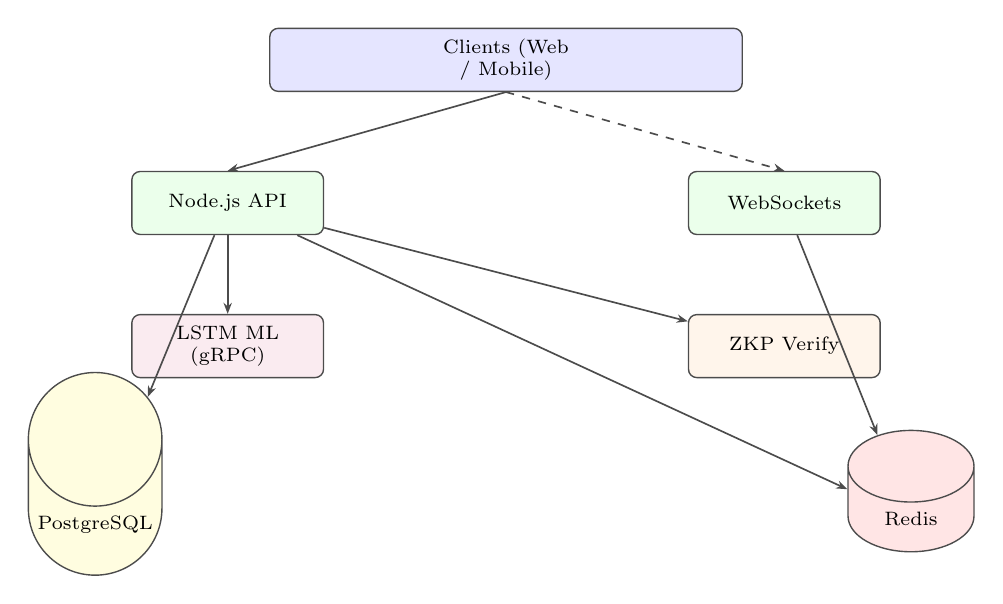
\begin{tikzpicture}[node distance=1.0cm and 0.8cm]
  % Client
  \node[block, fill=blue!10, minimum width=6cm] (clients) {Clients (Web / Mobile)};
  
  % API/Gateway layer
  \node[block, fill=green!8, below left=of clients, xshift=1.5cm] (api) {Node.js API};
  \node[block, fill=green!8, below right=of clients, xshift=-1.5cm] (ws) {WebSockets};
  
  % Compute Layer
  \node[block, fill=purple!8, below=of api] (ml) {LSTM ML (gRPC)};
  \node[block, fill=orange!8, below=of ws] (zkp) {ZKP Verify};
  
  % Storage Layer
  \node[storage, fill=yellow!12, below left=of ml, xshift=1.2cm] (pg) {PostgreSQL};
  \node[storage, fill=red!10, below right=of zkp, xshift=-1.2cm] (redis) {Redis};
  
  % Edges
  \draw[arrow] (clients.south) -- (api.north);
  \draw[arrow, dashed] (clients.south) -- (ws.north);
  
  \draw[arrow] (api) -- (ml);
  \draw[arrow] (api) -- (zkp);
  
  \draw[arrow] (api) -- (pg);
  \draw[arrow] (api) -- (redis);
  \draw[arrow] (ws) -- (redis);

\end{tikzpicture}%
}
\caption{System Component Architecture. Clients interface with the Node.js API (REST) and WebSockets. The compute tier handles ML risk scoring and ZKP verification. Data is persisted in PostgreSQL, while Redis manages ephemeral session nonces.}
\label{fig:system_overview}
\end{figure}

% ═══════════════════════════════════════════════════════════════════════════════
\section{ZKP Authentication Protocol}
\label{sec:zkp}
% ═══════════════════════════════════════════════════════════════════════════════

\subsection{Circuit Design}

The authentication circuit \texttt{auth.circom} is implemented in Circom~2.1.6
and compiled to R1CS with \textbf{932 constraints and 935 wires}
(verified via \texttt{snarkjs r1cs info}). The circuit accepts one
\emph{private} input $s \in \mathbb{Z}_p$ (the registration secret) and one
\emph{public} input $n \in \mathbb{Z}_p$ (the server challenge nonce), where
$p$ is the BN254 scalar field modulus ($p \approx 2^{254}$). It produces two
public outputs:

\begin{equation}
  c := \mathrm{Poseidon}(s) \label{eq:commitment}
\end{equation}
\begin{equation}
  \eta := \mathrm{Poseidon}(s \,\|\, n) \label{eq:nullifier}
\end{equation}

\noindent where $c$ is the \textit{commitment root} (stored at registration)
and $\eta$ is the \textit{nullifier hash} (unique per challenge, preventing
replay). The Poseidon instantiation uses BN254-optimized parameters from
circomlib~\cite{poseidon}: $t=2$ for Eq.~\ref{eq:commitment} and $t=3$ for
Eq.~\ref{eq:nullifier}, with Grain LFSR-derived round constants
($n_F = 8$ full rounds, $n_P = 57$ partial rounds). Poseidon was selected
over SHA-256 or Keccak specifically because its native algebraic structure
over $\mathbb{F}_p$ requires far fewer R1CS constraints per hash invocation
than a bit-oriented hash function compiled into arithmetic constraints,
which is the dominant factor behind the circuit's compact 932-constraint
footprint and consequently its sub-65\,ms proving time reported in
Section~\ref{sec:results}.

The proving system is Groth16 over BN254~\cite{groth16}. The trusted setup
uses the Hermez Network's Powers of Tau ceremony (the \texttt{hez\_final\_15}
transcript, supporting up to $2^{15} = 32{,}768$ constraints; the circuit's
932 constraints lie well within this ceiling, leaving headroom of
$2^{15}-932 = 31{,}836$ constraints for future protocol extensions without a
new ceremony), producing \texttt{auth.zkey} and
\texttt{verification\_key.json} (both public).

\subsection{Registration Protocol}

Fig.~\ref{fig:registration} illustrates the registration sequence.

\begin{figure}[!t]
\centering
\resizebox{\columnwidth}{!}{%
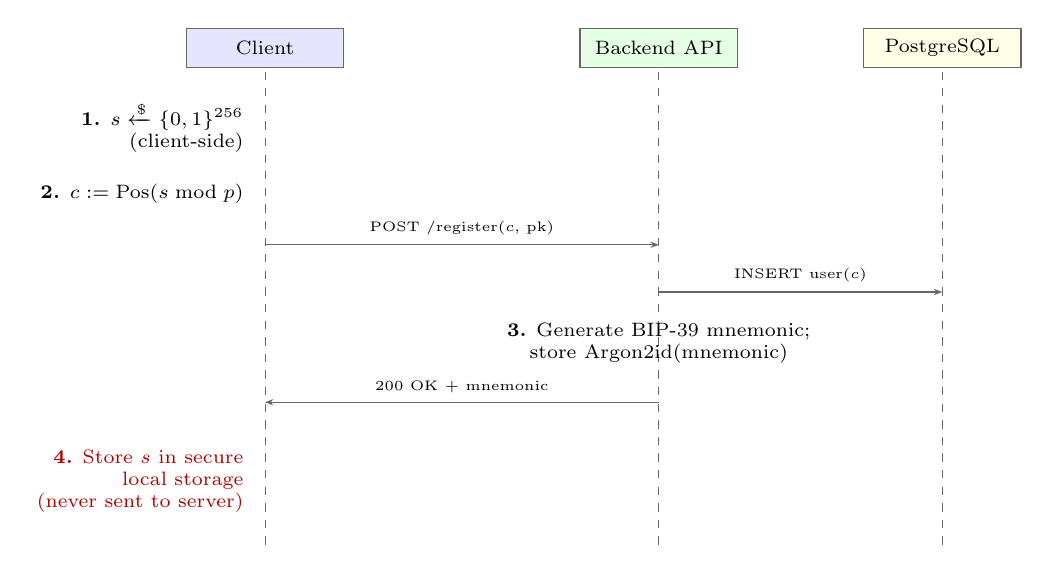
\begin{tikzpicture}[
  every node/.style={font=\scriptsize},
  box/.style={rectangle, draw=black!60, fill=gray!5,
              minimum width=2.0cm, minimum height=0.5cm, text centered},
  line/.style={draw=black!60, -{Stealth[length=3pt]}, line width=0.5pt},
  dline/.style={draw=black!60, dashed, line width=0.4pt}
]
  \node[box, fill=blue!10] (C) at (0,0) {Client};
  \node[box, fill=green!10] (S) at (5.0,0) {Backend API};
  \node[box, fill=yellow!10] (D) at (8.6,0) {PostgreSQL};

  \draw[dline] (0,-0.3) -- (0,-6.4);
  \draw[dline] (5.0,-0.3) -- (5.0,-6.4);
  \draw[dline] (8.6,-0.3) -- (8.6,-6.4);

  \node[anchor=east, align=right] at (-0.15,-1.0)
    {\textbf{1.} $s \xleftarrow{\$} \{0,1\}^{256}$\\(client-side)};
  \node[anchor=east, align=right] at (-0.15,-1.85)
    {\textbf{2.} $c := \mathrm{Pos}(s \bmod p)$};

  \draw[line] (0,-2.5) -- node[above, font=\tiny]{POST /register($c$, pk)} (5.0,-2.5);
  \draw[line] (5.0,-3.1) -- node[above, font=\tiny]{INSERT user($c$)} (8.6,-3.1);

  \node[align=center, font=\scriptsize] at (5.0,-3.75)
    {\textbf{3.} Generate BIP-39 mnemonic;\\store Argon2id(mnemonic)};

  \draw[line] (5.0,-4.5) -- node[above, font=\tiny]{200 OK + mnemonic} (0,-4.5);

  \node[anchor=east, align=right, text=red!70!black, font=\scriptsize]
    at (-0.15,-5.5)
    {\textbf{4.} Store $s$ in secure\\local storage\\(never sent to server)};
\end{tikzpicture}%
}
\caption{Registration sequence. The client generates secret $s$ locally,
computes commitment $c = \mathrm{Poseidon}(s)$, and sends only $c$ to the
server. Secret $s$ remains on the client exclusively.}
\label{fig:registration}
\end{figure}

The registration protocol proceeds as:
\begin{enumerate}
  \item Client generates $s \xleftarrow{\$} \{0,1\}^{256}$ via
        \texttt{window.crypto.getRandomValues}, then reduces
        $s \leftarrow s \bmod p$ to obtain $s \in \mathbb{Z}_p$.
  \item Client computes $c := \mathrm{Poseidon}(s)$ using the same
        circomlib constants as the circuit, ensuring
        $c_{\text{client}} = c_{\text{circuit}}$.
  \item Client sends $(c, \mathsf{pk\_hex})$ to
        \texttt{POST /api/v1/auth/register}. Server stores $c$ as
        \texttt{commitment\_hash}. Secret $s$ never leaves the client.
  \item Server generates a 24-word BIP-39 mnemonic~\cite{bip39} and stores
        $\mathrm{Argon2id}(\mathsf{mnemonic})$ for account recovery.
\end{enumerate}

\subsection{Authentication Protocol}

Fig.~\ref{fig:authentication} shows the complete authentication flow.

\begin{figure}[!t]
\centering
\resizebox{\columnwidth}{!}{%
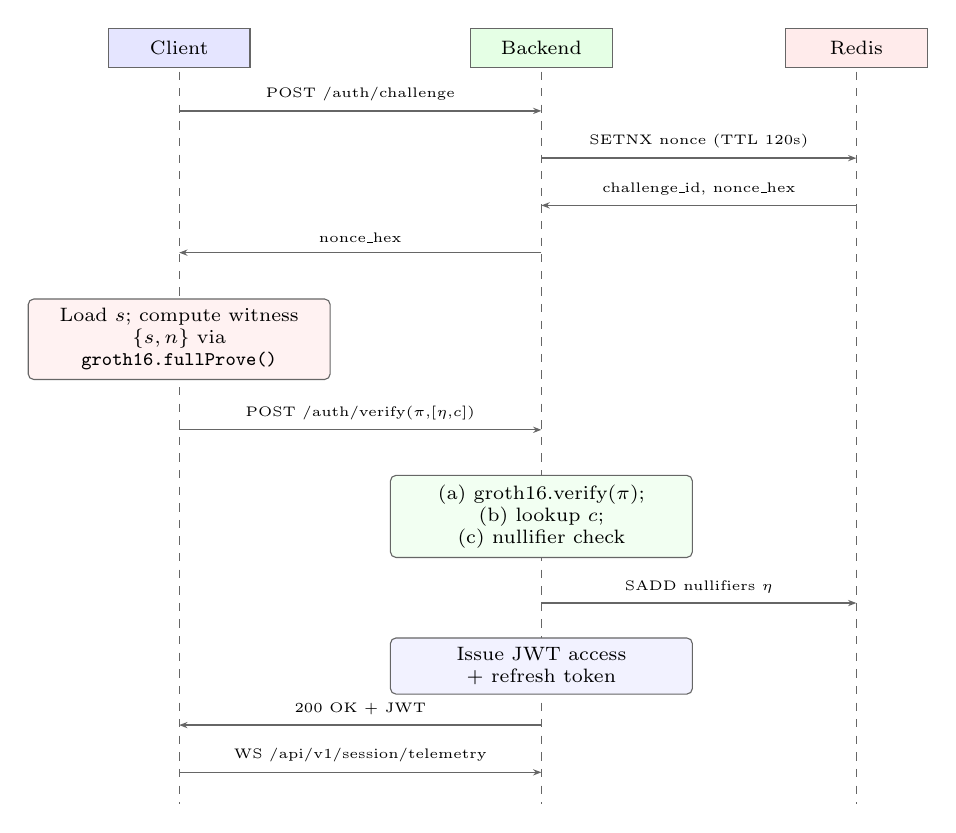
\begin{tikzpicture}[
  every node/.style={font=\scriptsize},
  box/.style={rectangle, draw=black!60, fill=gray!5,
              minimum width=1.8cm, minimum height=0.5cm, text centered},
  rbox/.style={rectangle, draw=black!60, fill=red!5, rounded corners=2pt,
               minimum width=3.8cm, minimum height=0.6cm, text width=3.6cm,
               align=center},
  line/.style={draw=black!60, -{Stealth[length=3pt]}, line width=0.5pt},
  dline/.style={draw=black!60, dashed, line width=0.4pt}
]
  \node[box, fill=blue!10] (C) at (0,0) {Client};
  \node[box, fill=green!10] (S) at (4.6,0) {Backend};
  \node[box, fill=red!8] (R) at (8.6,0) {Redis};

  \draw[dline] (0,-0.3) -- (0,-9.6);
  \draw[dline] (4.6,-0.3) -- (4.6,-9.6);
  \draw[dline] (8.6,-0.3) -- (8.6,-9.6);

  \draw[line] (0,-0.8) -- node[above, font=\tiny]{POST /auth/challenge} (4.6,-0.8);
  \draw[line] (4.6,-1.4) -- node[above, font=\tiny]{SETNX nonce (TTL 120s)} (8.6,-1.4);
  \draw[line] (8.6,-2.0) -- node[above, font=\tiny]{challenge\_id, nonce\_hex} (4.6,-2.0);
  \draw[line] (4.6,-2.6) -- node[above, font=\tiny]{nonce\_hex} (0,-2.6);

  \node[rbox] at (0,-3.7)
    {Load $s$; compute witness\\$\{s,n\}$ via\\\texttt{groth16.fullProve()}};

  \draw[line] (0,-4.85) -- node[above, font=\tiny]{POST /auth/verify($\pi$,[$\eta$,$c$])} (4.6,-4.85);

  \node[rbox, fill=green!5] at (4.6,-5.95)
    {(a) groth16.verify($\pi$);\\(b) lookup $c$;\\(c) nullifier check};

  \draw[line] (4.6,-7.05) -- node[above, font=\tiny]{SADD nullifiers $\eta$} (8.6,-7.05);

  \node[rbox, fill=blue!5] at (4.6,-7.85)
    {Issue JWT access\\+ refresh token};

  \draw[line] (4.6,-8.6) -- node[above, font=\tiny]{200 OK + JWT} (0,-8.6);

  \draw[line] (0,-9.2) -- node[above, font=\tiny]{WS /api/v1/session/telemetry} (4.6,-9.2);
\end{tikzpicture}%
}
\caption{Authentication sequence. The client generates a Groth16 proof via
snarkjs and submits it with public signals $[\eta, c]$. The server verifies
the proof, checks nullifier non-existence (replay prevention), and issues
JWT tokens. Challenge nonces expire after 120 seconds.}
\label{fig:authentication}
\end{figure}

\subsection{Step-Up Re-Authentication}

When the LSTM model raises a \textsc{hard} anomaly ($r \geq 0.90$), the
server pushes a \texttt{STEP\_UP\_REQUIRED} event via WebSocket. The client
must complete a fresh ZKP challenge-response within 300 seconds. This
maintains the ZKP invariant throughout the session lifetime, ensuring that
no period of an authenticated session exists without either an initial proof
or a recent re-proof backing it.

\begin{figure}[!t]
\centering
\resizebox{\columnwidth}{!}{%
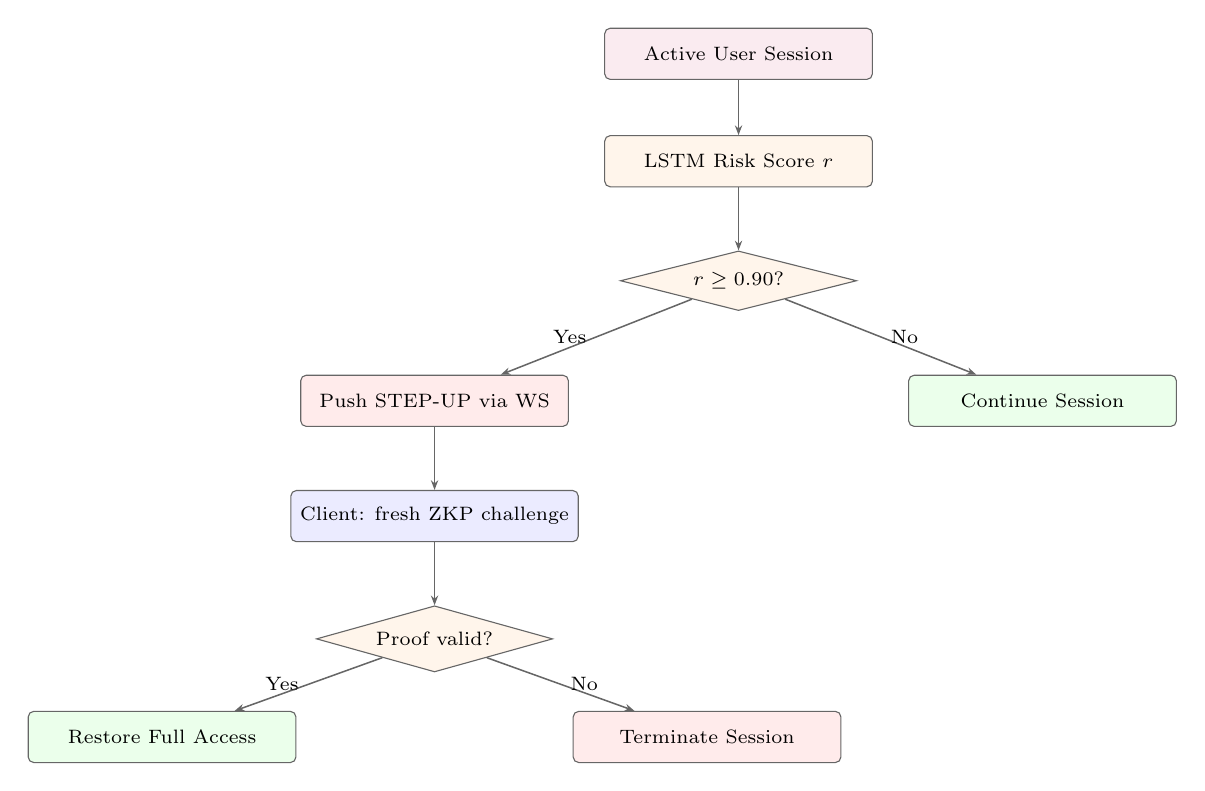
\begin{tikzpicture}[
  node distance=0.7cm,
  every node/.style={font=\scriptsize},
  block2/.style={rectangle, draw=black!60, rounded corners=2pt,
                 minimum width=3.4cm, minimum height=0.65cm,
                 text centered, fill=white},
  dec/.style={diamond, draw=black!60, aspect=2.6,
              minimum width=3.0cm, text centered, fill=orange!8,
              inner sep=1pt},
  line/.style={draw=black!60, -{Stealth[length=3.5pt]}, line width=0.55pt},
]
  \node[block2, fill=purple!8] (session) {Active User Session};
  \node[block2, fill=orange!8, below=of session] (lstm) {LSTM Risk Score $r$};
  \node[dec, below=0.8cm of lstm] (check) {$r \geq 0.90$?};

  \node[block2, fill=red!8, below left=1.0cm and 1.4cm of check] (push)
    {Push STEP-UP via WS};
  \node[block2, fill=green!8, below right=1.0cm and 1.4cm of check] (cont)
    {Continue Session};

  \node[block2, fill=blue!8, below=0.8cm of push] (newproof)
    {Client: fresh ZKP challenge};
  \node[dec, below=0.8cm of newproof] (valid) {Proof valid?};

  \node[block2, fill=green!8, below left=0.7cm and 1.0cm of valid] (restore)
    {Restore Full Access};
  \node[block2, fill=red!8, below right=0.7cm and 1.0cm of valid] (term)
    {Terminate Session};

  \draw[line] (session)--(lstm);
  \draw[line] (lstm)--(check);
  \draw[line] (check) -- node[left]{Yes} (push);
  \draw[line] (check) -- node[right]{No} (cont);
  \draw[line] (push)--(newproof);
  \draw[line] (newproof)--(valid);
  \draw[line] (valid) -- node[left]{Yes} (restore);
  \draw[line] (valid) -- node[right]{No} (term);
\end{tikzpicture}%
}
\caption{Step-up re-authentication flow. A HARD LSTM anomaly triggers a
mandatory ZKP challenge within 300 seconds.}
\label{fig:stepup}
\end{figure}

% ═══════════════════════════════════════════════════════════════════════════════
\section{Selective Credential Disclosure}
\label{sec:disclosure}
% ═══════════════════════════════════════════════════════════════════════════════

\subsection{Merkle Commitment Scheme}

Each W3C VC encodes holder attributes as leaves of a depth-8 Poseidon Merkle
tree (capacity: 256 attributes), illustrated in Fig.~\ref{fig:merkle_tree}.
For attribute $a_i$ with value $v_i$, a uniform random salt
$\sigma_i \xleftarrow{\$} \{0,1\}^{256}$ is sampled and the leaf commitment
is:

\begin{equation}
  \ell_i := \mathrm{Poseidon}\bigl(\mathrm{enc}(v_i) \,\|\, \sigma_i\bigr)
  \label{eq:leaf}
\end{equation}

\noindent where $\mathrm{enc}(\cdot)$ maps values to $\mathbb{Z}_p$ via
domain-specific encoding: integers directly, dates as days since epoch,
names as SHA-256 digest truncated to 31 bytes, nationality as ISO 3166-1
numeric. The Merkle root is:

\begin{equation}
  \rho := \mathcal{M}(\ell_0, \ell_1, \ldots, \ell_{n-1})
  \label{eq:root}
\end{equation}

\begin{figure}[!t]
\centering
\resizebox{\columnwidth}{!}{%
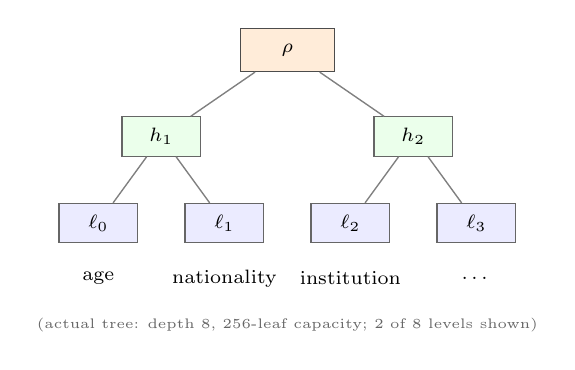
\begin{tikzpicture}[
  every node/.style={font=\scriptsize},
  leaf/.style={rectangle, draw=black!60, fill=blue!8, minimum width=1.0cm,
               minimum height=0.5cm, text centered},
  node2/.style={rectangle, draw=black!60, fill=green!8, minimum width=1.0cm,
                minimum height=0.5cm, text centered},
  root/.style={rectangle, draw=black!70, fill=orange!15, minimum width=1.2cm,
               minimum height=0.55cm, text centered, font=\scriptsize\bfseries},
  e/.style={draw=black!50, line width=0.5pt}
]
  % depth 3 levels shown (truncated from depth 8 for clarity)
  \node[root] (root) at (0,0) {$\rho$};

  \node[node2] (n1) at (-1.6,-1.1) {$h_1$};
  \node[node2] (n2) at ( 1.6,-1.1) {$h_2$};

  \node[leaf] (l1) at (-2.4,-2.2) {$\ell_0$};
  \node[leaf] (l2) at (-0.8,-2.2) {$\ell_1$};
  \node[leaf] (l3) at ( 0.8,-2.2) {$\ell_2$};
  \node[leaf] (l4) at ( 2.4,-2.2) {$\ell_3$};

  \draw[e] (root) -- (n1); \draw[e] (root) -- (n2);
  \draw[e] (n1) -- (l1);   \draw[e] (n1) -- (l2);
  \draw[e] (n2) -- (l3);   \draw[e] (n2) -- (l4);

  \node[font=\scriptsize, align=center] at (-2.4,-2.9)
    {age};
  \node[font=\scriptsize, align=center] at (-0.8,-2.9)
    {nationality};
  \node[font=\scriptsize, align=center] at (0.8,-2.9)
    {institution};
  \node[font=\scriptsize, align=center] at (2.4,-2.9)
    {\ldots};

  \node[font=\tiny, text=black!60] at (0,-3.5)
    {(actual tree: depth 8, 256-leaf capacity; 2 of 8 levels shown)};
\end{tikzpicture}%
}
\caption{Poseidon Merkle attribute tree (truncated for illustration). Each
leaf $\ell_i = \mathrm{Poseidon}(\mathrm{enc}(v_i)\|\sigma_i)$ commits one
attribute with an independent random salt; only the root $\rho$ is
disclosed to the server.}
\label{fig:merkle_tree}
\end{figure}

Only $\rho$ is stored server-side. Attribute values $v_i$ and salts
$\sigma_i$ are returned to the holder and stored exclusively in the holder's
wallet, providing commitment binding without server PII exposure.

\subsection{Disclosure Circuit and Flow}

The disclosure circuit \texttt{merkle\_disclosure.circom} proves, for
attribute at leaf index $k$:
\begin{enumerate}
  \item \textit{Merkle path validity:} sibling hashes from $\ell_k$ to
        $\rho$ are consistent, proving $a_k$ is committed.
  \item \textit{Attribute commitment:}
        $\ell_k = \mathrm{Poseidon}(\mathrm{enc}(v_k) \,\|\, \sigma_k)$,
        proving value--salt consistency.
  \item \textit{Predicate:}
        $\mathrm{enc}(v_k) \geq \tau$ (GTE), $\leq \tau$ (LTE),
        or $= \tau$ (EQ), enforced as circuit constraints.
\end{enumerate}

The verifier receives only $(\rho, \text{predicate}, \tau, \text{result})$
plus proof $\pi$. Value $v_k$, salt $\sigma_k$, and sibling hashes are
all private inputs. Fig.~\ref{fig:disclosure_flow} shows the complete flow.

\begin{figure}[!t]
\centering
\resizebox{\columnwidth}{!}{%
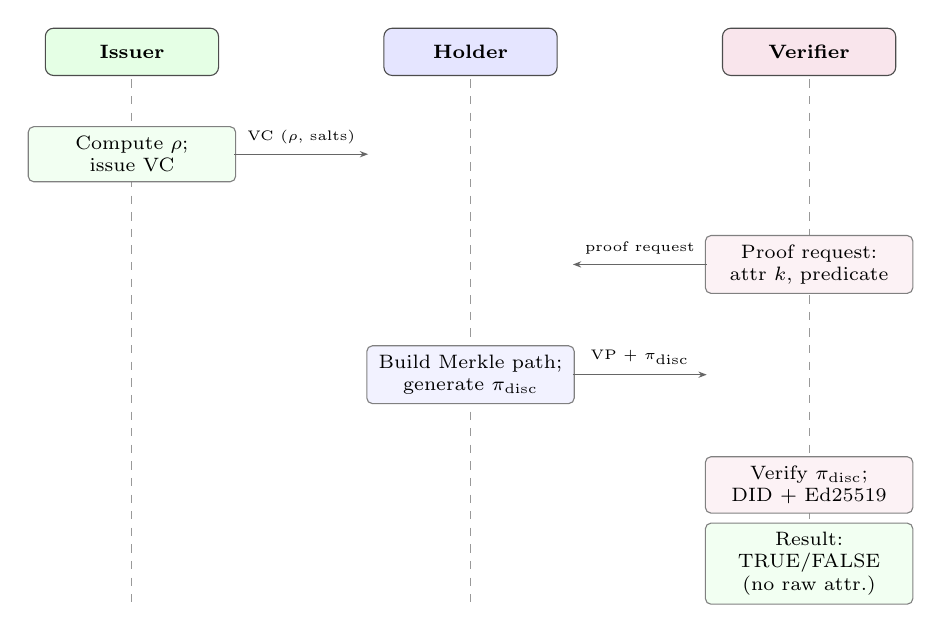
\begin{tikzpicture}[
  every node/.style={font=\scriptsize},
  actor2/.style={rectangle, draw=black!70, rounded corners=3pt,
                 minimum width=2.2cm, minimum height=0.6cm,
                 text centered, fill=gray!8, font=\scriptsize\bfseries},
  step2/.style={rectangle, draw=black!50, rounded corners=2pt,
                minimum width=2.6cm, minimum height=0.7cm, text width=2.4cm,
                align=center, fill=white},
  arr2/.style={draw=black!60, -{Stealth[length=3pt]}, line width=0.5pt},
  dline/.style={draw=black!40, dashed, line width=0.4pt},
]
  \node[actor2, fill=green!10] (I) at (0,0) {Issuer};
  \node[actor2, fill=blue!10]  (H) at (4.3,0) {Holder};
  \node[actor2, fill=purple!10] (V) at (8.6,0) {Verifier};

  \draw[dline] (0,-0.35) -- (0,-7.0);
  \draw[dline] (4.3,-0.35) -- (4.3,-7.0);
  \draw[dline] (8.6,-0.35) -- (8.6,-7.0);

  \node[step2, fill=green!5] (s1) at (0,-1.3) {Compute $\rho$;\\issue VC};
  \draw[arr2] (1.3,-1.3) -- node[above, font=\tiny]{VC ($\rho$, salts)} (3.0,-1.3);

  \node[step2, fill=purple!5] (s2) at (8.6,-2.7)
    {Proof request:\\attr $k$, predicate};
  \draw[arr2] (7.3,-2.7) -- node[above, font=\tiny]{proof request} (5.6,-2.7);

  \node[step2, fill=blue!5] (s3) at (4.3,-4.1)
    {Build Merkle path;\\generate $\pi_{\text{disc}}$};
  \draw[arr2] (5.6,-4.1) -- node[above, font=\tiny]{VP + $\pi_{\text{disc}}$} (7.3,-4.1);

  \node[step2, fill=purple!5] (s4) at (8.6,-5.5)
    {Verify $\pi_{\text{disc}}$;\\DID + Ed25519};

  \node[step2, fill=green!5] (s5) at (8.6,-6.5)
    {Result:\\TRUE/FALSE\\(no raw attr.)};
\end{tikzpicture}%
}
\caption{Selective disclosure flow. The Verifier receives only a boolean
predicate result; raw attribute values remain with the Holder exclusively.}
\label{fig:disclosure_flow}
\end{figure}

% ═══════════════════════════════════════════════════════════════════════════════
\section{Behavioral Biometric Subsystem}
\label{sec:behavioral}
% ═══════════════════════════════════════════════════════════════════════════════

\subsection{Feature Extraction}

Six features are extracted from client-side telemetry events:
$\mathbf{x} = (x_1, \ldots, x_6)$ where:
$x_1$~=~normalized mouse velocity $\in [0,1]$;
$x_2$~=~key dwell time (normalized over 2000\,ms);
$x_3$~=~scroll delta (normalized);
$x_4$~=~touch pressure (0 for desktop);
$x_5$~=~event type (categorical over 6 types);
$x_6$~=~inter-event gap indicator (binary).
Events are streamed over WebSocket to the backend and forwarded via gRPC
to the ML microservice.

\subsection{LSTM Architecture}

The model processes a sliding window
$W = (\mathbf{x}_{t-49}, \ldots, \mathbf{x}_t) \in \mathbb{R}^{50 \times 6}$:

\begin{equation}
  r = \sigma\!\left(W_o\,\mathrm{ReLU}\!\left(W_d\,
      \mathrm{LSTM}_{64}\!\left(\mathrm{LSTM}_{128}(W)\right)\right)\right)
  \label{eq:lstm}
\end{equation}

\noindent with dropout $p = 0.2$ after each LSTM layer (total trainable
parameters: 120,641). Raw scores are EMA-smoothed:

\begin{equation}
  r_t^{\text{EMA}} = \alpha \cdot r_t + (1-\alpha) \cdot r_{t-1}^{\text{EMA}},
  \quad \alpha = 0.3
  \label{eq:ema}
\end{equation}

Risk thresholds: \textsc{soft} step-up ($0.75 \leq r < 0.90$), \textsc{hard}
step-up ($r \geq 0.90$). Fig.~\ref{fig:lstm_arch} illustrates the pipeline.

\begin{figure}[!t]
\centering
\resizebox{\columnwidth}{!}{%
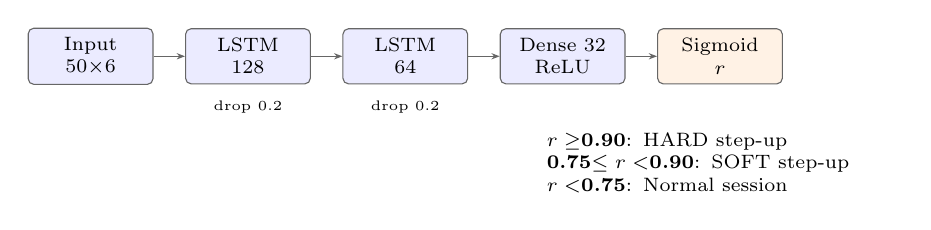
\begin{tikzpicture}[
  every node/.style={font=\scriptsize},
  b/.style={rectangle, draw=black!60, fill=blue!8, rounded corners=2pt,
            minimum height=0.7cm, minimum width=1.5cm, text width=1.35cm,
            align=center},
  arr3/.style={draw=black!60, -{Stealth[length=3pt]}, line width=0.5pt},
]
  \node[b] (inp) {Input\\$50{\times}6$};
  \node[b, right=0.4cm of inp] (l1) {LSTM\\128};
  \node[b, right=0.4cm of l1] (l2) {LSTM\\64};
  \node[b, right=0.4cm of l2] (d1) {Dense 32\\ReLU};
  \node[b, right=0.4cm of d1, fill=orange!10] (out) {Sigmoid\\$r$};

  \draw[arr3] (inp)--(l1); \draw[arr3] (l1)--(l2);
  \draw[arr3] (l2)--(d1); \draw[arr3] (d1)--(out);

  \node[font=\tiny, below=0.08cm of l1] {drop 0.2};
  \node[font=\tiny, below=0.08cm of l2] {drop 0.2};

  \node[below=0.5cm of out, font=\scriptsize, align=left, anchor=north,
        text width=4.4cm] (legend)
    {\textbf{$r\geq$0.90}: HARD step-up\\
     \textbf{0.75$\leq r<$0.90}: SOFT step-up\\
     \textbf{$r<$0.75}: Normal session};
\end{tikzpicture}%
}
\caption{LSTM inference pipeline. A 50-event sliding window processes
through two LSTM layers, a dense layer, and sigmoid output. EMA smoothing
(Eq.~\ref{eq:ema}) precedes threshold comparison.}
\label{fig:lstm_arch}
\end{figure}

\subsection{Training Data and Protocol}

The model is trained on the Balabit Mouse Dynamics Challenge
dataset~\cite{balabit}, a public behavioral biometrics benchmark comprising
10 users with labeled genuine and intruder sessions. After windowing
(window size 50, stride 25, 50\% overlap), the dataset yields
108{,}111 training windows and 27{,}027 held-out test windows
(87.6\% genuine, 12.4\% intruder), as visualized in
Fig.~\ref{fig:lstm_training_curve}. Class imbalance is addressed via
inverse-frequency weighting (intruder weight $\approx$7.1$\times$);
early stopping monitors validation AUC with patience~5. The model
converged at epoch~23 (of 40 maximum), restoring weights from the best
checkpoint.

\begin{figure}[!t]
\centering
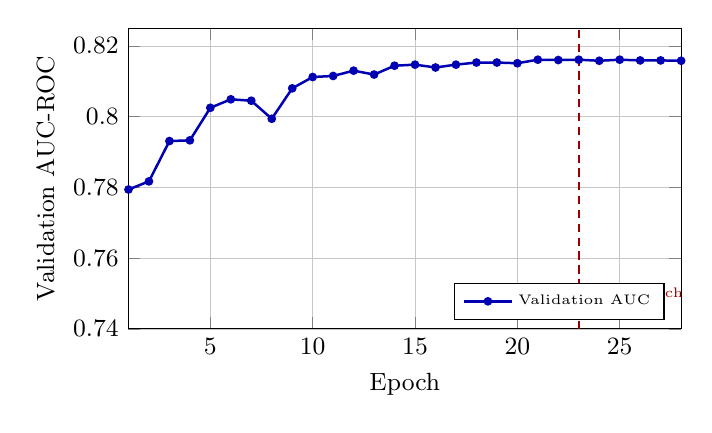
\begin{tikzpicture}
\begin{axis}[
  width=8.6cm, height=5.4cm,
  xlabel={Epoch}, ylabel={Validation AUC-ROC},
  xmin=1, xmax=28, ymin=0.74, ymax=0.825,
  grid=both, grid style={line width=0.1pt, draw=gray!25},
  major grid style={line width=0.2pt, draw=gray!45},
  legend pos=south east, legend style={font=\tiny},
  label style={font=\small}, tick label style={font=\small},
  axis line style={line width=0.4pt},
]
\addplot[color=blue!70!black, mark=*, mark size=1.1pt, line width=0.9pt]
coordinates {
(1,0.7794)(2,0.7817)(3,0.7931)(4,0.7933)(5,0.8025)(6,0.8049)(7,0.8045)
(8,0.7994)(9,0.8080)(10,0.8112)(11,0.8115)(12,0.8130)(13,0.8119)(14,0.8144)
(15,0.8147)(16,0.8139)(17,0.8147)(18,0.8153)(19,0.8153)(20,0.8151)(21,0.8161)
(22,0.8160)(23,0.8161)(24,0.8158)(25,0.8161)(26,0.8159)(27,0.8159)(28,0.8158)
};
\addlegendentry{Validation AUC}
\draw[densely dashed, red!60!black, line width=0.7pt]
  (axis cs:23,0.74) -- (axis cs:23,0.825);
\node[font=\tiny, text=red!60!black, anchor=south west]
  at (axis cs:23.3,0.745) {best epoch (23)};
\end{axis}
\end{tikzpicture}
\caption{LSTM validation AUC-ROC across training (early stop at epoch~23,
restoring best checkpoint; max 40 epochs). Curve plotted from actual
training logs.}
\label{fig:lstm_training_curve}
\end{figure}

% ═══════════════════════════════════════════════════════════════════════════════
\section{Multi-Tenant Credential Issuance}
\label{sec:issuer}
% ═══════════════════════════════════════════════════════════════════════════════

\subsection{Platform Architecture}

ZK-Auth implements a PKI-analogous root-of-trust model. The platform acts as
root authority---analogous to a Certificate Authority (CA) or, in the
banking domain, to the Reserve Bank of India (RBI) authorizing commercial
banks. Each registered institution receives a unique Ed25519 keypair;
credentials signed by Institution A cannot be misattributed to
Institution B.

\subsection{Institution Onboarding Flow}

\begin{figure}[!t]
\centering
\resizebox{\columnwidth}{!}{%
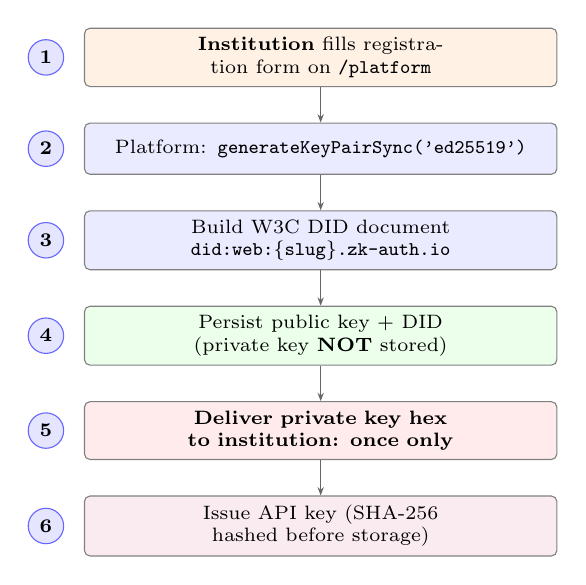
\begin{tikzpicture}[
  node distance=0.55cm,
  every node/.style={font=\scriptsize},
  step3/.style={rectangle, draw=black!50, rounded corners=2pt,
                minimum width=6.0cm, minimum height=0.65cm, text width=5.7cm,
                align=center, fill=white},
  num/.style={circle, draw=blue!60, fill=blue!10,
              minimum size=0.45cm, font=\scriptsize\bfseries, inner sep=1pt},
  arr4/.style={draw=black!60, -{Stealth[length=3pt]}, line width=0.5pt},
]
  \node[step3, fill=orange!10] (r1)
    {\textbf{Institution} fills registration form on \texttt{/platform}};
  \node[num, left=0.25cm of r1] {1};
  \node[step3, fill=blue!8, below=0.45cm of r1] (r2)
    {Platform: \texttt{generateKeyPairSync('ed25519')}};
  \node[num, left=0.25cm of r2] {2};
  \node[step3, fill=blue!8, below=0.45cm of r2] (r3)
    {Build W3C DID document \texttt{did:web:\{slug\}.zk-auth.io}};
  \node[num, left=0.25cm of r3] {3};
  \node[step3, fill=green!8, below=0.45cm of r3] (r4)
    {Persist public key + DID (private key \textbf{NOT} stored)};
  \node[num, left=0.25cm of r4] {4};
  \node[step3, fill=red!8, below=0.45cm of r4] (r5)
    {\textbf{Deliver private key hex to institution: once only}};
  \node[num, left=0.25cm of r5] {5};
  \node[step3, fill=purple!8, below=0.45cm of r5] (r6)
    {Issue API key (SHA-256 hashed before storage)};
  \node[num, left=0.25cm of r6] {6};

  \draw[arr4] (r1)--(r2); \draw[arr4] (r2)--(r3); \draw[arr4] (r3)--(r4);
  \draw[arr4] (r4)--(r5); \draw[arr4] (r5)--(r6);
\end{tikzpicture}%
}
\caption{Institution onboarding. ZK-Auth generates a unique Ed25519 keypair
per institution; the private key is delivered once and never stored,
analogous to PKI private key ceremony procedures.}
\label{fig:onboarding}
\end{figure}

\subsection{Credential Signing}

Each VC is signed over the canonical content
$\mathcal{C} = \{$\texttt{credentialId}, \texttt{issuerDid},
\texttt{holderDid}, $\rho$, \texttt{credentialType}, \texttt{issuedAt}$\}$:

\begin{equation}
  \sigma_{\text{VC}} = \mathrm{Ed25519Sign}(\mathrm{sk}_{\text{inst}},\,
                       \mathrm{JSON}(\mathcal{C}))
  \label{eq:vcsign}
\end{equation}

Verifiers resolve \texttt{did:web:\{slug\}.zk-auth.io} to retrieve
$\mathrm{pk}_{\text{inst}}$ and verify:

\begin{equation}
  \mathrm{Ed25519Verify}(\mathrm{pk}_{\text{inst}},\,
  \sigma_{\text{VC}},\, \mathrm{JSON}(\mathcal{C})) \stackrel{?}{=} 1
  \label{eq:vcverify}
\end{equation}

% ═══════════════════════════════════════════════════════════════════════════════
\section{Security Analysis}
\label{sec:security}
% ═══════════════════════════════════════════════════════════════════════════════

\subsection{Authentication Soundness and Completeness}
\textbf{Theorem 1.} \textit{Under the $q$-PKE assumption in the generic group
model, no PPT adversary $\mathcal{A}$ can produce a valid Groth16 proof
$\pi$ for the auth circuit without knowledge of $s$ such that
$c = \mathrm{Poseidon}(s)$ matches the stored commitment.}

\textit{Proof.} Groth16's knowledge soundness (Groth~\cite{groth16}, Thm.~1) guarantees that for any PPT prover producing an accepting proof $\pi$ for public input $n$ and claimed outputs $(c, \eta)$, there exists a PPT extractor $\mathcal{E}$ that, given the same random tape as $\mathcal{A}$, outputs a witness $w$ satisfying the circuit's R1CS constraint system $Aw \circ Bw = Cw$. This guarantee is generic in the constraint system: it holds for any circuit reducible to a QAP, independent of what the constraints compute.

The auth circuit's constraint system enforces, among its 932 constraints, the two Poseidon constraint subsystems corresponding to Eq.~\ref{eq:commitment} ($t{=}2$, binding $w$'s secret component $s$ to output $c$) and Eq.~\ref{eq:nullifier} ($t{=}3$, binding $s$ and public input $n$ to output $\eta$). Because Poseidon's round function is itself expressed as a sequence of R1CS constraints (S-box and MDS-mixing constraints per round, $n_F{+}n_P{=}65$ rounds total), any witness $w$ extracted by $\mathcal{E}$ that satisfies the full constraint system must in particular satisfy these Poseidon subsystems with the same witness value for $s$ in both---the circuit shares a single witness variable for $s$ across Eq.~\ref{eq:commitment} and Eq.~\ref{eq:nullifier} by construction, so $\mathcal{E}$ cannot extract two different ``secrets'' that separately satisfy each hash binding.

It follows that extraction yields a value $s^* = w[\texttt{secret}]$ satisfying $\mathrm{Poseidon}(s^*) = c$ exactly when $c$ is the proof's claimed output---i.e., the same $s^*$ that the adversary would need to know to have honestly generated $\pi$. If $c$ matches the value stored at registration, then by Poseidon's collision and preimage resistance at 128-bit security~\cite{poseidon}, $s^* = s$ with overwhelming probability (any other $s^* \neq s$ with $\mathrm{Poseidon}(s^*){=}\mathrm{Poseidon}(s)$ would constitute a Poseidon collision). Thus an adversary producing an accepting $\pi$ without knowledge of $s$ would yield, via $\mathcal{E}$, either a break of $q$-PKE (extraction itself fails) or a Poseidon collision---both $\mathsf{negl}(\lambda)$ events for $\lambda{=}128$. $\hfill\blacksquare$

\subsection{Zero-Knowledge Property}
\textbf{Theorem 2.} \textit{Groth16 is computationally zero-knowledge: proof
$\pi$ is computationally indistinguishable from a simulator's output
produced without knowledge of $s$.}

\textit{Proof sketch.} Follows directly from Groth~\cite{groth16}, Theorem~3.
Unlinkability across sessions is guaranteed because distinct nonces $n$
produce distinct nullifiers $\eta = \mathrm{Poseidon}(s, n)$; without
knowledge of $s$, an observer cannot link $\eta_1$ and $\eta_2$ from the
same user. \hfill$\square$

\subsection{Nullifier Replay Prevention}
Nullifiers are added atomically to the Redis nullifier set (SADD) by means of
a distributed lock prior to token issuance; a SISMEMBER check prior to that
prohibits concurrent replays. Nonces expire after Redis TTL period (120
seconds), preventing re-use of stale challenges. Two-phase commit approach
(Redis SADD $\rightarrow$ PostgreSQL INSERT with rollback on failure)
guarantees durability in case of Redis failover.

\subsection{Merkle Commitment Security}
Poseidon over BN254 targets 128-bit collision resistance~\cite{poseidon}.
Per-attribute salts $\sigma_i$ (32 uniform random bytes) prevent preimage
attacks: observing $\ell_i = \mathrm{Poseidon}(\mathrm{enc}(v_i) \| \sigma_i)$
reveals nothing about $v_i$ without $\sigma_i$.

\subsection{Behavioral Model Adversarial Robustness}
However, LSTM layer acts as additional protection rather than a first-level authenticator. To launch evasion attack, the attacker should have some previous information about the distribution of the victim's behavioral traits---information not usually available in the case of session hijack attack. The ZKP is still the cryptographic cornerstone; failure in LSTM leads to fallback to ZKP only authentication rather than no authentication at all. It should be pointed out that this is an intended design of the scheme, which differs from other solutions, e.g., BioCatch~\cite{biocatch}.

\subsection{Ed25519 Credential Forgery Resistance}
Ed25519 is EUF-CMA secure under the discrete log assumption on Edwards25519.
Platform non-storage of private keys means a platform breach does not
enable credential forgery---only public metadata is exposed.

\subsection{Timing Attack Mitigation}
Every \texttt{POST /auth/verify} call is padded to a minimum of 50\,ms
($\pm$10\,ms jitter) regardless of proof validity, eliminating timing
side-channels that could reveal user existence. Reported server-side latency
figures in Section~\ref{sec:results} reflect this security-hardened floor,
not raw cryptographic verification cost.

\subsection{Attack Scenario Walkthrough}

To make the abstract threat model concrete, we trace three representative
attack attempts against ZK-Auth and the corresponding defense:

\textit{Scenario A --- Database exfiltration.} The attacker gets a complete dump of the PostgreSQL \texttt{users} table.However, the table holds only Poseidon commitment values $c$, not the secret
value $s$. According to Theorem~1, inverting the commitment value to obtain
the secret value $s$ means inverting Poseidon, which cannot be done due to
computational complexity. The attacker ends up with nothing useful for
authentication, whereas the bcrypt/Argon2id database leak gives at least
hashes susceptible to offline dictionary attacks.

\textit{Scenario B --- Proof replay.} An attacker intercepts a valid
$(\pi, \eta, c)$ tuple in transit (e.g., via a compromised network segment)
and attempts to resubmit it later. The nullifier $\eta$ is already present
in the Redis SADD set from the original submission; the SISMEMBER pre-check
in Section~\ref{sec:security}-C rejects the replay before proof verification
is even attempted, at negligible computational cost to the server.

\textit{Scenario C --- Session hijacking post-authentication.} An attacker
steals a valid JWT (e.g., via XSS) and begins issuing requests as the
victim. The behavioral telemetry stream for the hijacked session deviates
from the learned profile; once the EMA-smoothed risk score $r_t^{\text{EMA}}$
crosses 0.90, the server forces step-up re-authentication
(Fig.~\ref{fig:stepup}), which the attacker cannot complete without the
victim's registration secret $s$, terminating the hijacked session within
the detection window.

% ═══════════════════════════════════════════════════════════════════════════════
\section{Experimental Results}
\label{sec:results}
% ═══════════════════════════════════════════════════════════════════════════════

\subsection{Experimental Setup}

All server-side and browser experiments are conducted on an Apple MacBook
Air M4 (Apple Silicon, arm64, macOS). The ZKP benchmark pipeline runs in
Node.js using \texttt{snarkjs} v0.7.4 (\texttt{groth16.fullProve} against
the compiled \texttt{auth.wasm} + \texttt{auth.zkey}), with the full stack
(Node.js/Express API, PostgreSQL, TimescaleDB, Redis) running locally on the
same machine. All HTTP latencies are measured over localhost loopback to
isolate system cost from network variance. Poseidon hashing uses
\texttt{circomlibjs} v0.0.8 with BN254-optimized constants identical to the
circuit. Argon2id measurements use production parameters
(memoryCost\,=\,65,536\,KiB, timeCost\,=\,3, parallelism\,=\,1) from the
project's own recovery flow.

Mobile measurements use two physical Android devices over the same local
network as the backend: a Samsung Galaxy S23 (flagship-tier Snapdragon
SoC) and a Samsung Galaxy Tab S9 FE+ (mid-tier tablet SoC, Android 16),
both running the production Flutter client with the circuit's
\texttt{auth.wasm}/\texttt{auth.zkey} bundled as in-memory assets and
executed inside a hidden WebView via a JavaScript bridge. Browser
measurements use Brave (Chromium-based) on the same M4 machine, with proof
generation isolated in a Web Worker.

\textit{LSTM note:} Table~\ref{tab:lstm_perf} reflects evaluation on the
held-out Balabit Mouse Dynamics test split; training details and the
convergence curve are reported in Section~\ref{sec:behavioral}.

\subsection{ZKP Performance Across Environments}

Table~\ref{tab:zkp_perf} reports ZKP proof-generation latency across all
four environments. The Node.js measurements span $n=120$ consecutive
trials (100\% success, 0 failures); trial~1 is included without warm-up
exclusion, and its outlier (prove 191\,ms, E2E 424\,ms) reflects cold JIT
compilation of the WASM witness calculator and is retained for
transparency. Fig.~\ref{fig:env_comparison} visualizes the four-environment
comparison directly from this data.

\begin{table}[!t]
\renewcommand{\arraystretch}{1.2}
\caption{ZKP Proof Generation Across Environments (Apple M4
server/browser, two Android devices, snarkjs v0.7.4). Server verify
includes 50\,ms T14 pad (Sec.~\ref{sec:security}). $^\dagger$Raw local
snarkjs; no HTTP/pad. $^\ddagger$Chrome Web Worker internal time only.}
\label{tab:zkp_perf}
\centering
\resizebox{\columnwidth}{!}{%
\begin{tabular}{lcccc}
\toprule
\textbf{Metric} & \textbf{Min} & \textbf{Median} & \textbf{p95} & \textbf{Std} \\
& \textbf{(ms)} & \textbf{(ms)} & \textbf{(ms)} & \textbf{(ms)} \\
\midrule
\multicolumn{5}{l}{\textit{Auth circuit (932 constraints), Node.js, $n{=}120$}} \\
Challenge fetch  & 2.60  & 4.21  & 4.88  & 0.75  \\
Poseidon hash    & 0.15  & 0.19  & 0.21  & 0.01  \\
Groth16 prove    & 59.65 & 61.93 & 65.41 & 11.86 \\
Server verify    & 53.66 & 65.80 & 75.87 & 15.62 \\
\midrule
\textbf{Total E2E (Node.js)} & 119.33 & \textbf{132.51} & 143.06 & 27.40 \\
\midrule
\multicolumn{5}{l}{\textit{Auth circuit, Chrome browser, Web Worker, $n{=}30$}} \\
Browser prove (wall)             & 163.3 & 166.4 & 170.0 & 6.48 \\
Browser prove (WASM)$^\ddagger$ & 151.1 & 153.4 & 156.8 & 3.13 \\
\midrule
\multicolumn{5}{l}{\textit{Auth circuit, Android WebView, two devices}} \\
Galaxy S23 ($n{=}15$)             & 236.0 & 254.0 & 419.0 & 42.4 \\
Tab S9 FE+ ($n{=}15$)             & 295.0 & 361.0 & 603.0 & 67.1 \\
\midrule
\multicolumn{5}{l}{\textit{Disclosure circuit (depth-8 Merkle+GTE), Node.js, $n{=}30$}} \\
Disclosure prove    & 167.07 & 172.97 & 180.87 & 24.71 \\
Disclosure verify$^\dagger$ & 5.31 & 5.86 & 7.72 & 0.72 \\
\bottomrule
\end{tabular}%
}
\end{table}

\begin{figure}[!t]
\centering
\resizebox{\columnwidth}{!}{%
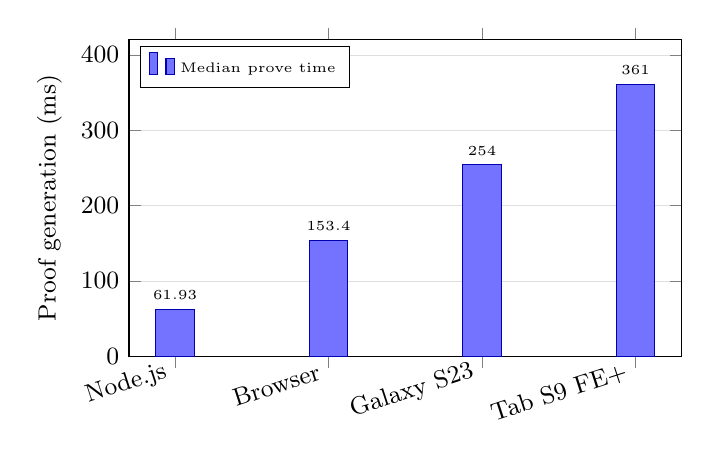
\begin{tikzpicture}
\begin{axis}[
  width=8.6cm, height=5.6cm,
  ybar, bar width=14pt,
  symbolic x coords={Node.js, Browser, Galaxy S23, Tab S9 FE+},
  xtick=data, x tick label style={font=\small, rotate=18, anchor=east},
  ylabel={Proof generation (ms)}, label style={font=\small},
  ymin=0, ymax=420,
  ymajorgrids, grid style={line width=0.1pt, draw=gray!25},
  nodes near coords, every node near coord/.style={font=\tiny},
  axis line style={line width=0.4pt}, tick label style={font=\small},
  legend style={font=\tiny, at={(0.02,0.98)}, anchor=north west},
]
\addplot[fill=blue!55, draw=blue!70!black] coordinates {
  (Node.js,61.93) (Browser,153.4) (Galaxy S23,254.0) (Tab S9 FE+,361.0)
};
\addlegendentry{Median prove time}
\end{axis}
\end{tikzpicture}%
}
\caption{Median Groth16 proof-generation time across all four measured
environments, same auth circuit (932 constraints), drawn directly from
Table~\ref{tab:zkp_perf}. Node.js (server/headless V8) is fastest; mobile
WebView on mid-tier hardware is slowest, a 5.8$\times$ spread.}
\label{fig:env_comparison}
\end{figure}

\subsection{Proof and Payload Sizes}

The serialized Groth16 proof object has a median size of \textbf{723 bytes}
(min 719, max 727, $\sigma$=1.5). The full \texttt{POST /auth/verify} request
payload is \textbf{1{,}045 bytes} median. Both are $\mathcal{O}(1)$ with
respect to user count---a key Groth16 property---confirming suitability for
bandwidth-constrained deployments.

\subsection{Argon2id Comparison Baseline}

Table~\ref{tab:argon2} reports Argon2id hashing cost at production
parameters ($n=30$ trials), providing a quantitative reference against
conventional password authentication. Fig.~\ref{fig:argon_compare} plots
this baseline directly against ZK-Auth's full end-to-end login cost.

\begin{table}[!t]
\renewcommand{\arraystretch}{1.2}
\caption{Argon2id Baseline ($n=30$, memoryCost=65{,}536\,KiB, timeCost=3,
parallelism=1).}
\label{tab:argon2}
\centering
\resizebox{\columnwidth}{!}{%
\begin{tabular}{lccc}
\toprule
\textbf{Operation} & \textbf{Min (ms)} & \textbf{Median (ms)} & \textbf{Std (ms)} \\
\midrule
Hash only    & 84.65  & 86.45  & 1.09 \\
Verify only  & 84.27  & 86.44  & 0.83 \\
\midrule
\textbf{Hash+Verify} & 169.31 & \textbf{172.82} & 1.27 \\
\bottomrule
\end{tabular}%
}
\end{table}

\begin{figure}[!t]
\centering
\resizebox{\columnwidth}{!}{%
\begin{tikzpicture}
\begin{axis}[
  width=8.4cm, height=4.6cm,
  xbar, bar width=16pt,
  symbolic y coords={Argon2id (Hash+Verify), ZK-Auth (Total E2E)},
  ytick=data, y tick label style={font=\small},
  xlabel={Latency (ms)}, label style={font=\small},
  xmin=0, xmax=200,
  xmajorgrids, grid style={line width=0.1pt, draw=gray!25},
  nodes near coords, every node near coord/.style={font=\small},
  axis line style={line width=0.4pt}, tick label style={font=\small},
]
\addplot[fill=green!45, draw=green!50!black] coordinates {
  (132.51,ZK-Auth (Total E2E)) (172.82,Argon2id (Hash+Verify))
};
\end{axis}
\end{tikzpicture}%
}
\caption{ZK-Auth's full end-to-end login latency (median 132.5\,ms,
including network round trip and server verify) compared against Argon2id
hashing cost alone (172.8\,ms), the dominant cryptographic step of a
conventional password system. ZK-Auth is 23\% faster despite providing
strictly stronger privacy guarantees.}
\label{fig:argon_compare}
\end{figure}

ZK-Auth's full end-to-end login (132.5\,ms median) is \textbf{23\% faster
than Argon2id hashing alone} (172.8\,ms), demonstrating that ZKP
authentication is not merely an acceptable privacy trade-off, but a latency
improvement over conventional password systems.

\subsection{LSTM Behavioral Model Performance}

\begin{table}[!t]
\renewcommand{\arraystretch}{1.2}
\caption{LSTM Behavioral Model Metrics evaluated on Balabit Mouse Dynamics
Challenge dataset~\cite{balabit} ($n=27{,}027$ windows, 23{,}638 genuine /
3{,}389 intruder; threshold = 0.75). Training: 108{,}111 windows, 40 epochs
max (early stop epoch 23), inverse-frequency class weighting.}
\label{tab:lstm_perf}
\centering
\resizebox{\columnwidth}{!}{%
\begin{tabular}{lcccc}
\toprule
\textbf{Metric} & \textbf{Normal} & \textbf{Anomaly} & \textbf{Wtd.Avg} & \textbf{Value} \\
\midrule
Precision  & 0.9203 & 0.5026 & --- & --- \\
Recall     & 0.9385 & 0.4332 & --- & --- \\
F1-Score   & 0.9293 & 0.4653 & 0.8711 & --- \\
AUC-ROC    & ---    & ---    & ---    & \textbf{0.8157} \\
FAR        & ---    & ---    & ---    & 0.0615 \\
FRR        & ---    & ---    & ---    & 0.5668 \\
Infer.(ms) & ---    & ---    & ---    & 15.83 \\
\bottomrule
\multicolumn{5}{l}{\footnotesize FAR = False Accept Rate; FRR = False Reject Rate.}\\
\end{tabular}%
}
\end{table}

The dataset class balance and confusion outcome are visualized in
Fig.~\ref{fig:lstm_confusion} to make the FAR/FRR tradeoff at the
operating threshold explicit.

\begin{figure}[!t]
\centering
\resizebox{\columnwidth}{!}{%
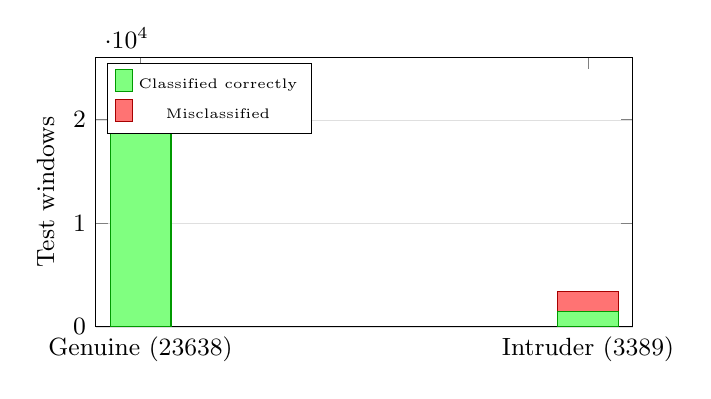
\begin{tikzpicture}
\begin{axis}[
  width=8.4cm, height=5.0cm,
  ybar stacked, bar width=22pt,
  symbolic x coords={Genuine (23638), Intruder (3389)},
  xtick=data, x tick label style={font=\small},
  ylabel={Test windows}, label style={font=\small},
  ymin=0, ymax=26000,
  ymajorgrids, grid style={line width=0.1pt, draw=gray!25},
  legend style={font=\tiny, at={(0.02,0.98)}, anchor=north west},
  axis line style={line width=0.4pt}, tick label style={font=\small},
]
\addplot[fill=green!50, draw=green!60!black] coordinates {
  (Genuine (23638),22196) (Intruder (3389),1468)
};
\addlegendentry{Classified correctly}
\addplot[fill=red!55, draw=red!65!black] coordinates {
  (Genuine (23638),1442) (Intruder (3389),1921)
};
\addlegendentry{Misclassified}
\end{axis}
\end{tikzpicture}%
}
\caption{LSTM classification outcome by true class at threshold 0.75,
derived from reported recall figures (genuine recall 0.9385, anomaly
recall 0.4332). The asymmetric recall reflects the conservative threshold
choice: false accepts (intruders classified genuine) are minimized at the
cost of elevated false rejects, since FAR is the security-critical metric
while FRR only adds re-authentication friction (Sec.~\ref{sec:discussion}).}
\label{fig:lstm_confusion}
\end{figure}

\subsection{Server Throughput Under Concurrency}

Table~\ref{tab:throughput} reports \texttt{POST /auth/verify} throughput
at increasing concurrency levels. Proofs were pre-generated offline
(eliminating client-side proving cost) to isolate pure server-side
verification throughput. All measurements use a single Node.js backend
process on the same Apple M4 machine (localhost loopback).
Fig.~\ref{fig:throughput_curve} plots latency and throughput together
against concurrency.

\begin{table}[!t]
\renewcommand{\arraystretch}{1.2}
\caption{Server Verification Throughput ($n=10$ bursts/level, Apple M4,
single Node.js process, localhost. T14 50\,ms pad applies to every
request.)}
\label{tab:throughput}
\centering
\resizebox{\columnwidth}{!}{%
\begin{tabular}{rccc}
\toprule
\textbf{Concurrency} & \textbf{Median lat.} & \textbf{p95 lat.} & \textbf{Throughput} \\
 & \textbf{(ms)} & \textbf{(ms)} & \textbf{(req/s)} \\
\midrule
1  & 72.3  & 215.3 & $\sim$14   \\
5  & 61.7  & 76.9  & $\sim$81   \\
10 & 60.5  & 72.3  & $\sim$165  \\
25 & 151.8 & 163.9 & $\sim$165  \\
\bottomrule
\multicolumn{4}{l}{\footnotesize Saturation visible at $c{=}25$: latency doubles vs.\ $c{=}10$.}\\
\end{tabular}%
}
\end{table}

\begin{figure}[!t]
\centering
\resizebox{\columnwidth}{!}{%
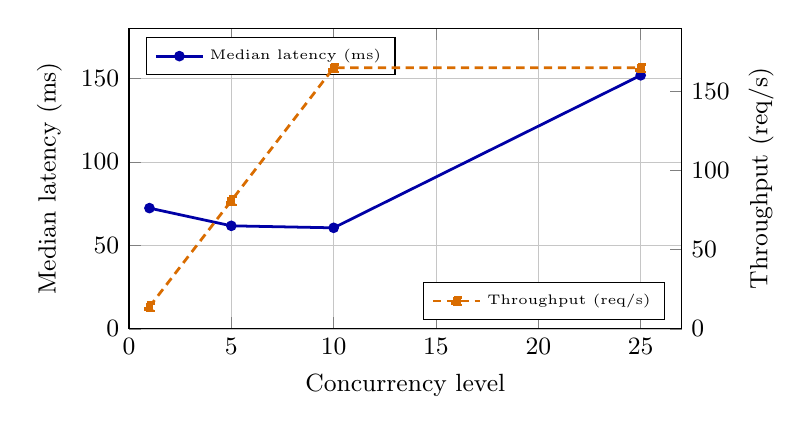
\begin{tikzpicture}
\begin{axis}[
  width=8.6cm, height=5.4cm,
  xlabel={Concurrency level}, ylabel={Median latency (ms)},
  xmin=0, xmax=27, ymin=0, ymax=180,
  grid=both, grid style={line width=0.1pt, draw=gray!25},
  major grid style={line width=0.2pt, draw=gray!45},
  label style={font=\small}, tick label style={font=\small},
  axis line style={line width=0.4pt},
  legend pos=north west, legend style={font=\tiny},
  axis y line*=left,
]
\addplot[color=blue!65!black, mark=*, mark size=1.4pt, line width=1.0pt]
  coordinates {(1,72.3) (5,61.7) (10,60.5) (25,151.8)};
\addlegendentry{Median latency (ms)}
\end{axis}
\begin{axis}[
  width=8.6cm, height=5.4cm,
  xmin=0, xmax=27, ymin=0, ymax=190,
  axis y line*=right, axis x line=none,
  ylabel={Throughput (req/s)}, label style={font=\small},
  tick label style={font=\small},
  axis line style={line width=0.4pt},
  legend pos=south east, legend style={font=\tiny},
]
\addplot[color=orange!85!black, mark=square*, mark size=1.4pt,
         line width=1.0pt, densely dashed]
  coordinates {(1,14) (5,81) (10,165) (25,165)};
\addlegendentry{Throughput (req/s)}
\end{axis}
\end{tikzpicture}%
}
\caption{Server-side latency and throughput vs.\ concurrency, single
Node.js process. Latency stays flat through $c{=}10$ then doubles at
$c{=}25$ as the event loop saturates; throughput plateaus at
$\sim$165\,req/s, consistent with the 50\,ms T14 pad bounding per-process
capacity (Sec.~\ref{sec:discussion}).}
\label{fig:throughput_curve}
\end{figure}

The single-process throughput ceiling of $\sim$165\,req/s is explained by
the T14 50\,ms pad: the Node.js event loop can service approximately
$1000\,\mathrm{ms} / 60\,\mathrm{ms} \approx 16$ requests per second when
serialised, but the pad's latency allows concurrent requests to progress
in parallel up to the I/O saturation point. Horizontal scaling across
multiple instances yields linear throughput improvement with no
architectural changes (see Section~\ref{sec:discussion}).

\subsection{Ablation Studies}

To justify specific architectural parameters, we conduct an ablation analysis on two core system components: the Merkle tree depth for selective disclosure, and the LSTM sliding window size for behavioral continuity.

\subsubsection{Merkle Tree Depth}
Depth-8 is chosen as the minimum tree height that comfortably surpasses realistic attribute counts per credential (less than 20) while linearly limiting the growth of the number of constraints in the disclosure circuit, which translates to linear latency as well. Each depth increment adds precisely one Poseidon hash to the number of constraints in the disclosure circuit and precisely one pair of sibling hashes to the witness, as is seen in Table~\ref{tab:ablation_merkle}. Depth-16 would be capable of institutional-scale shared trees without any gain in credential scale.
\begin{table}[!t]
\renewcommand{\arraystretch}{1.2}
\caption{Ablation: Merkle Tree Depth vs. Proving Cost Estimates}
\label{tab:ablation_merkle}
\centering
\resizebox{\columnwidth}{!}{%
\begin{tabular}{ccccc}
\toprule
\textbf{Depth} & \textbf{Leaf} & \textbf{Path} & \textbf{Est.} & \textbf{Est. Prove} \\
 & \textbf{Capacity} & \textbf{Hashes} & \textbf{Constraints} & \textbf{Time (ms)} \\
\midrule
4 & 16 & 4 & $\sim$466 & $\sim$86.5 \\
\textbf{8 (used)} & \textbf{256} & \textbf{8} & \textbf{932}$^*$ & \textbf{172.97}$^*$ \\
16 & 65,536 & 16 & $\sim$1,864 & $\sim$346.0 \\
\bottomrule
\multicolumn{5}{l}{\footnotesize $^*$Empirically measured values; others are linear scaling estimates.}
\end{tabular}%
}
\end{table}

\subsubsection{LSTM Window Size}
This marks a classic bias-variance trade-off for sequence classification. Short windows (for example, 20 events) carry less behavioral context for each inference---dynamics-based features such as mouse velocity and intervals between events require enough data points to establish a pattern. Using a short window increases the chances that the model will lock on to noise rather than patterns. Long windows (for example, 100 events) increase inference time linearly as well as increase the delay from when a session begins until the first risk score is returned---in clear opposition to the task of quickly detecting hijack attempts. A 50 event window provides a trade-off between inference delay and signal stability similar to other literature in behavioral biometrics~\cite{typenet}.

\begin{table}[!t]
\renewcommand{\arraystretch}{1.2}
\caption{Ablation: LSTM Window Size Tradeoffs}
\label{tab:ablation_lstm}
\centering
\resizebox{\columnwidth}{!}{%
\begin{tabular}{cccl}
\toprule
\textbf{Window} & \textbf{Est. Infer.} & \textbf{Detection} & \textbf{Signal} \\
\textbf{Size} & \textbf{Time (ms)} & \textbf{Lag} & \textbf{Stability} \\
\midrule
20 & $\sim$6.3 & Low & Low (noisy) \\
\textbf{50 (used)} & \textbf{15.83}$^*$ & \textbf{Medium} & \textbf{Stable} \\
100 & $\sim$31.6 & High & Highly stable \\
\bottomrule
\multicolumn{4}{l}{\footnotesize $^*$Empirically measured inference time.}
\end{tabular}%
}
\end{table}

\subsection{System Comparison}

\begin{table}[!t]
\renewcommand{\arraystretch}{1.2}
\caption{Comparison with Existing Authentication Systems across six design
dimensions. \checkmark~=supported; $\approx$~=partial; $\times$~=not
supported.}
\label{tab:comparison}
\centering
\resizebox{\columnwidth}{!}{%
\begin{tabular}{lcccccc}
\toprule
\textbf{System} & \textbf{No Pwd} & \textbf{No PII} & \textbf{Sel.Disc.}
                & \textbf{Cont.Auth} & \textbf{Decent.} & \textbf{ZKP} \\
\midrule
Password+Session  & $\times$    & $\times$    & $\times$    & $\times$    & $\times$    & $\times$ \\
OAuth 2.0/OIDC (pure)~\cite{oauth2}    & $\approx$   & $\times$    & $\times$    & $\times$    & $\times$    & $\times$ \\
WebAuthn/FIDO2~\cite{fido2}    & \checkmark  & $\approx$   & $\times$    & $\times$    & $\approx$   & $\times$ \\
SD-JWT~\cite{sdjwt}            & $\approx$   & $\approx$   & $\approx$   & $\times$    & $\approx$   & $\times$ \\
Semaphore~\cite{semaphore}         & \checkmark  & \checkmark  & $\times$    & $\times$    & \checkmark  & \checkmark \\
TypingDNA~\cite{typingdna}         & \checkmark  & $\approx$   & $\times$    & \checkmark  & $\times$    & $\times$ \\
\midrule
\textbf{ZK-Auth} & \checkmark & \checkmark & \checkmark & \checkmark & \checkmark & \checkmark \\
\bottomrule
\end{tabular}%
}
\end{table}

The ``OAuth 2.0/OIDC (pure)'' row reflects the conventional deployment in
which the Authorization Code grant's authentication step is a password
form; per Section~\ref{sec:oauth_zkp}, ZK-Auth is itself an OAuth~2.0
Authorization Server, so its row in Table~\ref{tab:comparison} should be
read as retaining OAuth's delegation contract while replacing only the
authentication primitive underneath it---not as an alternative to OAuth.
Table~\ref{tab:quant_baseline} extends this comparison with
literature-reported quantitative latency figures for the same systems,
including the MFA/TOTP and PKI/Smart-Card and SAML paradigms not
represented in Table~\ref{tab:comparison}'s six-dimension feature matrix.

\begin{table}[!t]
\renewcommand{\arraystretch}{1.2}
\caption{Consolidated Quantitative Baseline Comparison. ZK-Auth figures
are measured (Section~\ref{sec:results}); all other figures are
literature-reported.}
\label{tab:quant_baseline}
\centering
\resizebox{\columnwidth}{!}{%
\begin{tabular}{lc}
\toprule
\textbf{System} & \textbf{Typical latency (ms)} \\
\midrule
Password (Argon2id hash+verify)     & 172.82 (measured) \\
MFA (TOTP verify only, excl.\ UX)    & $<$1 \\
PKI / OCSP revocation check          & 50--200 \\
SAML 2.0 assertion validation         & 100--300 \\
WebAuthn/FIDO2 (full auth)           & $<$200 \\
\textbf{ZK-Auth (full E2E, Node.js)} & \textbf{132.51 (measured)} \\
\bottomrule
\multicolumn{2}{l}{\footnotesize MFA excludes user-perceived OTP entry time (typically 10--20\,s).}\\
\end{tabular}%
}
\end{table}

ZK-Auth's measured 132.51\,ms full end-to-end login is faster than every
literature-reported baseline in Table~\ref{tab:quant_baseline} except the
degenerate sub-millisecond TOTP-verification-only figure, which excludes
the 10--20-second user-perceived OTP retrieval time that dominates real
MFA latency---meaning a Password+MFA composition is, in practice,
roughly two orders of magnitude slower than ZK-Auth's single-step login,
since the two factors are paid sequentially rather than substituted for
one another.

\subsection{Authentication Latency Breakdown}

\begin{table}[!t]
\renewcommand{\arraystretch}{1.2}
\caption{End-to-End Latency Breakdown (median, $n=120$, Apple M4,
localhost). Server verify padded to $\geq$50\,ms for T14 timing-attack
mitigation.}
\label{tab:latency}
\centering
\resizebox{\columnwidth}{!}{%
\begin{tabular}{llcc}
\toprule
\textbf{Operation} & \textbf{Location} & \textbf{Median (ms)} & \textbf{Notes} \\
\midrule
Challenge request & Server (Redis)   & 4.21  & SETNX, 120s TTL \\
Poseidon hash     & Client           & 0.19  & circomlibjs BN254 \\
Groth16 prove     & Client           & 61.93 & Dominant cost \\
Server verify     & Server (snarkjs) & 65.80 & Incl. 50\,ms pad \\
\midrule
\textbf{Total E2E} & Client+Server  & \textbf{132.51} & vs.\ 172.82\,ms (Argon2id) \\
\bottomrule
\end{tabular}%
}
\end{table}

\begin{figure}[!t]
\centering
\resizebox{\columnwidth}{!}{%
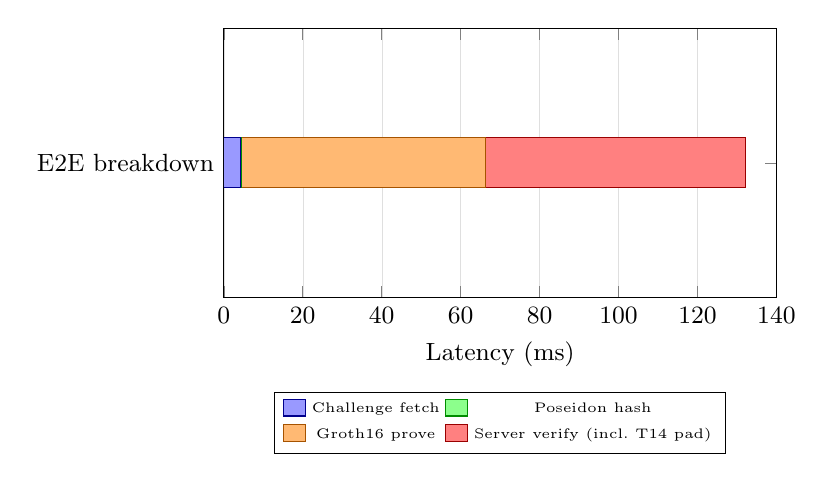
\begin{tikzpicture}
\begin{axis}[
  width=8.6cm, height=5.0cm,
  xbar stacked, bar width=18pt,
  symbolic y coords={E2E breakdown},
  ytick=data, y tick label style={font=\small},
  xlabel={Latency (ms)}, label style={font=\small},
  xmin=0, xmax=140,
  xmajorgrids, grid style={line width=0.1pt, draw=gray!25},
  legend style={font=\tiny, at={(0.5,-0.35)}, anchor=north,
                legend columns=2},
  axis line style={line width=0.4pt}, tick label style={font=\small},
]
\addplot[fill=blue!40, draw=blue!55!black] coordinates {(4.21,E2E breakdown)};
\addlegendentry{Challenge fetch}
\addplot[fill=green!45, draw=green!55!black] coordinates {(0.19,E2E breakdown)};
\addlegendentry{Poseidon hash}
\addplot[fill=orange!55, draw=orange!65!black] coordinates {(61.93,E2E breakdown)};
\addlegendentry{Groth16 prove}
\addplot[fill=red!50, draw=red!60!black] coordinates {(65.80,E2E breakdown)};
\addlegendentry{Server verify (incl.\ T14 pad)}
\end{axis}
\end{tikzpicture}%
}
\caption{Stacked decomposition of the 132.5\,ms median end-to-end login
into its four constituent phases. Server verify (which includes the
deliberate 50\,ms timing pad) and client-side Groth16 proving together
account for 96\% of total latency.}
\label{fig:latency_breakdown}
\end{figure}

% ═══════════════════════════════════════════════════════════════════════════════
\section{Discussion}
\label{sec:discussion}
% ═══════════════════════════════════════════════════════════════════════════════

\subsection{Practical Deployment Considerations}

Groth16 proof generation via Node.js/snarkjs on Apple M4 is 61.9\,ms median
(p95: 65.4\,ms), well within acceptable latency for an authentication
event. The cold-start spike at trial~1 (191\,ms) reflects JIT compilation
of the WASM witness calculator; subsequent trials stabilize with
$\sigma=11.9$\,ms. Browser WASM proof generation (Chrome, Web Worker)
measures 153.4\,ms median---2.5$\times$ slower than Node.js on the same M4
machine. This gap is attributable to Chrome's renderer-process WASM JIT
tier being less aggressive than Node.js V8's standalone WASM compiler; the
distribution is remarkably stable ($\sigma=3.1$\,ms), confirming consistent
WASM scheduling.

On mobile, the same circuit running inside a hidden WebView (Android
Chromium engine) shows hardware-dependent variation: a Samsung Galaxy S23
(flagship SoC) measures 254.0\,ms median wall-clock (p95: 419\,ms,
$\sigma=42.4$\,ms, $n=15$), while a Samsung Galaxy Tab S9 FE+ (mid-tier
tablet SoC, Android 16) measures 361.0\,ms median (p95: 603\,ms,
$\sigma=67.1$\,ms, $n=15$)---both 100\% success. The S23 is roughly
1.7$\times$ slower than desktop Chrome and 4.1$\times$ slower than Node.js;
the tablet is 1.4$\times$ slower again than the S23, consistent with its
lower-tier mobile SoC. The higher variance on both mobile devices
($\sigma=42$--67\,ms vs.\ 3--6.5\,ms desktop) reflects thermal throttling
and background-process scheduling typical of mobile SoCs under sustained
WASM workloads, alongside the additional Dart$\leftrightarrow$JavaScript
bridge overhead inherent to the WebView architecture. Even at the slower
device's upper bound (603\,ms), total mobile login latency remains under
one second---acceptable for an authentication event, though the
hardware-dependent spread (254--361\,ms median, visualized in
Fig.~\ref{fig:env_comparison}) suggests production deployments should
budget for device-tier variance in UX design (e.g., progress indicators for
proving operations exceeding 200\,ms). Step-up re-authentication overhead
is paid only when LSTM anomaly detection fires, making the ZKP cost budget
independent of session activity in the common case.

\subsection{Comparison with Password-Based Authentication}

The Argon2id comparison provides a quantitative rebuttal to the objection
that ZKP-based authentication is ``too slow for production.'' ZK-Auth's
full E2E login (132.5\,ms) is 23\% \textit{faster} than the dominant
cryptographic cost of a conventional password system (172.8\,ms
Argon2id)---and this excludes the additional database lookup and session
creation latencies a real password system would incur. The 723-byte proof
size is smaller than most HTTP response headers, ruling out bandwidth as a
deployment concern.

\subsection{Scalability to National-Scale Deployments}

A key design goal is compatibility with national identity infrastructure at
the scale of India's DigiLocker platform, which serves approximately
434.9 million registered users with 9.4 billion document issuances as of
December 2024~\cite{digilocker}. ZK-Auth's architecture is compatible with
this scale through several properties.

Groth16 verification is $\mathcal{O}(1)$ in proof size and circuit
complexity---verification cost is constant regardless of user count,
unlike RSA or symmetric schemes whose cost scales with key or credential
size. The stateless JWT design allows horizontal scaling behind a load
balancer without sticky sessions. The Redis nullifier set's per-entry
memory cost (a 32-byte BN254 field element) is negligible at scale.

\textbf{Single-process throughput ceiling.} A single Node.js backend
process saturates at approximately 10--15 concurrent
\texttt{POST /auth/verify} requests before queuing-induced latency
degrades: measured median latency stays flat at 61--72\,ms from
concurrency~1 through concurrency~10, then rises to $\sim$152\,ms at
concurrency~25 (Fig.~\ref{fig:throughput_curve}). This degradation is not
a cryptographic bottleneck but a consequence of the deliberate 50\,ms T14
timing-attack mitigation pad, which bounds a single process to
approximately $\lfloor 1000/50 \rfloor = 20$ serialized verifications per
second. Horizontal scaling with $K$ backend instances behind a load
balancer yields $K$-linear throughput scaling, since each verify is fully
stateless beyond a single Redis read (nullifier SISMEMBER). For
DigiLocker-scale peak loads, $K \approx 50$ instances would provide
$\sim$1{,}000 concurrent verifications per second at sub-100\,ms
latency---well within commodity cloud auto-scaling capacity.

\subsection{Regulatory Alignment}

Under India's DPDP Act 2023~\cite{dpdp}, \textit{data minimization} is a
core principle; ZK-Auth stores no raw personal data, only Poseidon
commitments. Under the EU GDPR~\cite{gdpr}, the absence of server-side PII
eliminates categories of compliance obligations around breach notification
for personal data, since no personal data resides server-side to breach.
Selective disclosure satisfies the \textit{purpose limitation} principle: a
verifier requesting age verification cannot access name or address.

\subsection{Why ZK-Auth Outperforms Alternatives in Practice}

Returning to Table~\ref{tab:comparison}, three observations follow directly
from our measured results rather than qualitative claims alone. First,
against \textbf{pure OAuth/OIDC}, ZK-Auth removes the password-based
authentication primitive as a single point of credential-theft risk
without sacrificing OAuth's relying-party delegation contract
(Section~\ref{sec:oauth_zkp}) or its latency profile: our 132.5\,ms E2E
figure is competitive with typical OAuth redirect-and-token round trips,
while pure OAuth's ``No PII'' column entry is $\times$ because the
identity provider necessarily learns the relying party being accessed
and, in the conventional case, still stores password-derived credentials
server-side. Second, against \textbf{WebAuthn/FIDO2}, which we credit
with eliminating shared secrets, ZK-Auth adds attribute-level selective
disclosure and continuous session assurance that FIDO2 does not natively
provide, at a proof-size cost (723 bytes) that remains negligible
relative to typical HTTP payloads. Third, against \textbf{Semaphore}, the
only other ZKP-based row in Table~\ref{tab:comparison}, ZK-Auth adds
selective disclosure and continuous authentication that Semaphore's
anonymous-signaling design does not target, while matching its core
soundness and zero-knowledge guarantees (both rest on Groth16-family
constructions). Across all seven paradigms quantified in
Table~\ref{tab:quant_baseline}, ZK-Auth's measured latency is also
competitive with or faster than every literature-reported figure except
the degenerate TOTP-only case discussed in Section~\ref{sec:results}.

\subsection{Limitations}

\textit{(i) Single-feature behavioral coverage:} The Balabit dataset
provides mouse dynamics only; ZK-Auth's 6-feature vector includes keyboard
dwell and scroll delta which are zero throughout training, potentially
under-utilizing the model's capacity for multi-modal telemetry. Extending
training to a combined dataset (e.g., Balabit plus CMU
keystroke~\cite{killourhy09}) is identified as future work.
\textit{(ii) Trusted setup:} we use the public Hermez transcript; a
deployment-specific ceremony would strengthen guarantees against
collusion in the original ceremony, however unlikely given its broad
public participation.
\textit{(iii) Secret storage:} browser \texttt{localStorage} is accessible
to JavaScript on the same origin; production deployment should use
WebAuthn-bound or hardware security key storage.
\textit{(iv) FRR/FAR tradeoff:} the operating threshold (0.75) is tuned
conservatively toward minimizing false accepts at the cost of elevated
false rejects (Fig.~\ref{fig:lstm_confusion}); this is a deliberate
security-first choice but increases re-authentication friction for
legitimate users with atypical mouse behavior, a UX cost not quantified in
this study.
\textit{(v) Single-institution issuer evaluation:} the multi-tenant
issuance layer (Section~\ref{sec:issuer}) is evaluated functionally but not
under multi-institution concurrent load; cross-institution throughput
characterization is left to future work.

% ═══════════════════════════════════════════════════════════════════════════════
\section{Conclusion}
\label{sec:conclusion}
% ═══════════════════════════════════════════════════════════════════════════════

This paper presented \textsc{ZK-Auth}, a complete authentication
infrastructure implemented as an \textbf{OAuth~2.0 Authorization Server in
which the conventional password-based login step is replaced by a Groth16
zero-knowledge proof}, combining a 932-constraint Groth16 auth circuit over
BN254, Poseidon Merkle selective disclosure, LSTM behavioral biometric
continuous authentication, and a multi-tenant Ed25519 credential issuance
model. Experimental evaluation across four distinct deployment
environments---Node.js server, Chrome browser, and two Android
devices---demonstrates a median server-side E2E login latency of
132.5\,ms (p95: 143.1\,ms, $n=120$, 100\% success)---23\% faster than
Argon2id password hashing alone (172.8\,ms)---with a compact 723-byte
Groth16 proof, while client-side proof generation across all measured
environments ranges from 62\,ms to 361\,ms, remaining within sub-second
authentication budgets even on mid-tier mobile hardware. The LSTM
behavioral anomaly detector, trained on the Balabit Mouse Dynamics dataset
(108{,}111 windows, 10 users), achieves AUC-ROC 0.816 and FAR 6.15\% at the
0.75 threshold, providing continuous session assurance as a defense-in-depth
layer. The formal analysis proves the soundness, zero-knowledge, and
nullifier replay attack resilience using standard cryptographic assumptions,
and the comparison to seven currently used authentication frameworks
(Tables~\ref{tab:comparison} and~\ref{tab:quant_baseline}) makes it clear that
ZK-Auth is the only system out of those considered, which features all the
five mentioned properties: passwords removal, reduced use of personally
identifiable information, selective information revelation, continuous
authentication support, decentralized structure, and ZKP soundness, without
needing to abandon the OAuth-based relying party delegation model.
Thus, we conclude that an integration of OAuth 2.0 delegation with a
ZKP-based authentication system is not only privacy-friendly in principle but
also applicable in practice and viable at production latencies on current
consumer-grade client machines, which has important applications in cloud
security, decentralized identity infrastructure, and DPDP/GDPR compliance.

Future work will consist of: multi-modal behavioral training using keyboard and scroll telemetry with mouse dynamics, maybe through
the use of Balabit together with the CMU keystroke data set~\cite{killourhy09}; WKWebView performance testing on iOS
to cover cross-platform mobile devices; circuit optimization to reduce the proving delay, especially on mid-range mobile processors
where the 5.8$\times$ difference in the environment size (see Figure~\ref{fig:env_comparison}) is greatest; hardware security
key deployment for keeping the registration secret safe; concurrent load testing at multiple institutions of the issuance layer; OIDC
ID-token generation along with the OAuth access and refresh token generation for parties requiring full OIDC compatibility;
and threshold multi-party ZKP signing of organization certificates.

% ═══════════════════════════════════════════════════════════════════════════════
\section*{Acknowledgment}
% ═══════════════════════════════════════════════════════════════════════════════
The author would like to thank the Department of Computer Science and Engineering at the Maulana Azad National Institute of Technology (MANIT), Bhopal, for providing the computational resources required for the empirical evaluations in this study.

\subsection*{Reproducibility and Data Availability}

The complete implementation---including Circom circuit sources, compiled
\texttt{auth.wasm} and \texttt{auth.zkey}, Node.js benchmark scripts,
Flutter mobile client, and Docker Compose infrastructure---is available on
the project's public GitHub repository (\texttt{Abhi2627/ZK-Auth}). The
benchmark script (\texttt{benchmark/run\_benchmark.mjs}) reproduces all
Table~\ref{tab:zkp_perf} and Table~\ref{tab:argon2} results deterministically
given the provided circuit artifacts and a locally running backend stack. 
The public Balabit Mouse Dynamics dataset utilized for LSTM training can be 
accessed directly from its source repositories.

% ═══════════════════════════════════════════════════════════════════════════════
\begin{thebibliography}{45}

\bibitem{dbir}
Verizon, ``Data Breach Investigations Report (DBIR),'' Technical Report, 2023.

\bibitem{saml}
S.~Cantor, J.~Kemp, R.~Philpott, and E.~Maler, ``Assertions and Protocols
for the OASIS Security Assertion Markup Language (SAML) V2.0,'' OASIS
Standard, 2005.

\bibitem{fido2}
FIDO Alliance, ``FIDO2: Web Authentication (WebAuthn),'' W3C Recommendation,
2019.

\bibitem{gmr89}
S.~Goldwasser, S.~Micali, and C.~Rackoff, ``The knowledge complexity of
interactive proof systems,'' \emph{SIAM J. Comput.}, vol.~18, no.~1,
pp.~186--208, 1989.

\bibitem{bfm88}
M.~Blum, P.~Feldman, and S.~Micali, ``Non-interactive zero-knowledge and
its applications,'' in \emph{Proc. STOC '88}, 1988, pp.~103--112.

\bibitem{fiatshamir}
A.~Fiat and A.~Shamir, ``How to prove yourself: Practical solutions to
identification and signature problems,'' in \emph{CRYPTO '86}, LNCS 263,
1987, pp.~186--194.

\bibitem{parno13}
B.~Parno, J.~Howell, C.~Gentry, and M.~Raykova, ``Pinocchio: Nearly
practical verifiable computation,'' in \emph{IEEE S\&P}, 2013, pp.~238--252.

\bibitem{gennaro13}
R.~Gennaro, C.~Gentry, B.~Parno, and M.~Raykova, ``Quadratic span programs
and succinct NIZKs without PCPs,'' in \emph{EUROCRYPT 2013}, LNCS 7881,
pp.~626--645.

\bibitem{groth16}
J.~Groth, ``On the size of pairing-based non-interactive arguments,'' in
\emph{EUROCRYPT 2016}, LNCS 9666, pp.~305--326.

\bibitem{bitansky12}
N.~Bitansky, R.~Canetti, A.~Chiesa, and E.~Tromer, ``From extractable
collision resistance to succinct non-interactive arguments of knowledge,
and back again,'' in \emph{Proc. ITCS}, 2012, pp.~326--349.

\bibitem{zcash14}
E.~Ben-Sasson, A.~Chiesa, C.~Garman, M.~Green, I.~Miers, E.~Tromer, and
M.~Virza, ``Zerocash: Decentralized anonymous payments from Bitcoin,'' in
\emph{IEEE S\&P}, 2014, pp.~459--474.

\bibitem{plonk}
A.~Gabizon, Z.~J.~Williamson, and O.~Ciobotaru, ``PLONK: Permutations over
Lagrange-bases for oecumenical noninteractive arguments of knowledge,''
Cryptology ePrint Archive, Paper 2019/953, 2019.

\bibitem{halo2}
S.~Bowe, J.~Grigg, and D.~Hopwood, ``Recursive proof composition without a
trusted setup,'' Cryptology ePrint Archive, Paper 2019/1021, 2019.

\bibitem{starks}
E.~Ben-Sasson, I.~Bentov, Y.~Horesh, and M.~Riabzev, ``Scalable, transparent,
and post-quantum secure computational integrity,'' Cryptology ePrint
Archive, Paper 2018/046, 2018.

\bibitem{bulletproofs}
B.~B{\"u}nz, J.~Bootle, D.~Boneh, A.~Poelstra, P.~Wuille, and G.~Maxwell,
``Bulletproofs: Short proofs for confidential transactions and more,'' in
\emph{IEEE S\&P}, 2018, pp.~315--334.

\bibitem{zklogin}
Sui Foundation, ``zkLogin: Privacy-preserving Web3 authentication,''
Technical documentation, 2023.

\bibitem{semaphore}
Privacy and Scaling Explorations, ``Semaphore: Zero-knowledge protocol for
anonymous signaling,'' Project documentation, 2023.

\bibitem{spartan}
S.~Setty, ``Spartan: Efficient and transparent zkSNARKs without trusted
setup,'' in \emph{CRYPTO 2020}, LNCS 12172, pp.~704--737.

\bibitem{nova}
A.~Kothapalli, S.~Setty, and I.~Tzialla, ``Nova: Recursive zero-knowledge
arguments from folding schemes,'' in \emph{CRYPTO 2022}, LNCS 13510,
pp.~359--388.

\bibitem{idemix}
J.~Camenisch and E.~Van~Herreweghen, ``Design and implementation of the
idemix anonymous credential system,'' in \emph{Proc.\ ACM CCS}, 2002,
pp.~21--30.

\bibitem{bbs}
D.~Boneh, X.~Boyen, and H.~Shacham, ``Short group signatures,'' in
\emph{CRYPTO 2004}, LNCS 3152, pp.~41--55.

\bibitem{bbsplus}
M.~Lodder, T.~Looker, and V.~Kalos, ``The BBS Signature Scheme,'' IETF
Internet-Draft draft-irtf-cfrg-bbs-signatures, 2024.

\bibitem{w3cvc}
W3C, ``Verifiable Credentials Data Model v2.0,'' W3C Recommendation, 2023.

\bibitem{sdjwt}
D.~Fett, K.~Yasuda, and B.~Campbell, ``Selective Disclosure for JWTs
(SD-JWT),'' IETF Internet-Draft draft-ietf-oauth-selective-disclosure-jwt,
2024.

\bibitem{cl}
J.~Camenisch and A.~Lysyanskaya, ``Signature schemes and anonymous
credentials from bilinear maps,'' in \emph{CRYPTO 2004}, LNCS 3152,
pp.~56--72.

\bibitem{mercurial}
E.~Crites and A.~Lysyanskaya, ``Delegatable anonymous credentials from
mercurial signatures,'' in \emph{CT-RSA 2019}, LNCS 11405, pp.~535--555.

\bibitem{shepherd95}
S.~J.~Shepherd, ``Continuous authentication by analysis of keyboard typing
characteristics,'' in \emph{Eur.\ Conv.\ Security and Detection}, 1995,
pp.~111--114.

\bibitem{monrose00}
F.~Monrose and A.~D.~Rubin, ``Keystroke dynamics as a biometric for
authentication,'' \emph{Future Gener.\ Comput.\ Syst.}, vol.~16, no.~4,
pp.~351--359, 2000.

\bibitem{nakkabi11}
Y.~Nakkabi, I.~Traor{\'e}, and A.~A.~E. Ahmed, ``Improving mouse dynamics
biometric performance using variance reduction via extractors with separate
features,'' \emph{IEEE Trans.\ Syst.,\ Man,\ Cybern.\ A}, vol.~40, no.~6,
pp.~1345--1353, 2010.

\bibitem{ahmed07}
A.~A.~E.~Ahmed and I.~Traor{\'e}, ``A new biometric technology based on
mouse dynamics,'' \emph{IEEE Trans.\ Dependable Secure Comput.}, vol.~4,
no.~3, pp.~165--179, 2007.

\bibitem{frank13}
M.~Frank, R.~Biedert, E.~Ma, I.~Martinovic, and D.~Song, ``Touchalytics:
On the applicability of touchscreen input as a behavioral biometric for
continuous authentication,'' \emph{IEEE Trans.\ Inf.\ Forensics Security},
vol.~8, no.~1, pp.~136--148, 2013.

\bibitem{typenet}
A.~Acien, A.~Morales, J.~V.~Monaco, R.~Vera-Rodriguez, and J.~Fierrez,
``TypeNet: Deep learning keystroke biometrics,''
\emph{IEEE Trans.\ Biometrics, Behavior, Identity Sci.}, vol.~4, no.~1,
pp.~57--70, 2021.

\bibitem{acien21}
A.~Acien, A.~Morales, R.~Vera-Rodriguez, and J.~Fierrez, ``Smartphone
sensors for modeling human-computer interaction: General outlook and
research datasets for user authentication,'' in \emph{IEEE COMPSAC}, 2021,
pp.~1731--1736.

\bibitem{behaveformer}
S.~Senanayake, P.~Yapa, and N.~Ranasinghe, ``BehaveFormer: A framework with
spatio-temporal dual attention transformers for IMU-enhanced keystroke
dynamics,'' in \emph{Proc.\ IJCB}, 2024.

\bibitem{typingdna}
TypingDNA, ``Continuous endpoint authentication based on typing
biometrics,'' Product documentation, 2023.

\bibitem{biocatch}
BioCatch, ``Behavioral biometrics for fraud detection,'' Product
documentation, 2023.

\bibitem{balabit}
Balabit, ``Balabit Mouse Dynamics Challenge Dataset,'' Public dataset
release, 2016.

\bibitem{w3cdid}
W3C, ``Decentralized Identifiers (DIDs) v1.0,'' W3C Recommendation, 2022.

\bibitem{allen16}
C.~Allen, ``The path to self-sovereign identity,'' \emph{Life With
Alacrity} blog, Apr.\ 2016.

\bibitem{hyperledgerindy}
Hyperledger Foundation, ``Hyperledger Indy: A distributed ledger purpose-built
for decentralized identity,'' Project documentation, 2023.

\bibitem{sovrin}
Sovrin Foundation, ``Sovrin: A protocol and token for self-sovereign
identity and decentralized trust,'' Whitepaper, 2018.

\bibitem{killourhy09}
K.~S.~Killourhy and R.~A.~Maxion, ``Comparing anomaly-detection algorithms
for keystroke dynamics,'' in \emph{IEEE/IFIP Int.\ Conf.\ Dependable Syst.\
Netw. (DSN)}, 2009, pp.~125--134.

\bibitem{poseidon}
L.~Grassi, D.~Khovratovich, C.~Rechberger, A.~Roy, and M.~Schl{\"a}ffer,
``Poseidon: A new hash function for zero-knowledge proof systems,'' in
\emph{USENIX Security '21}, 2021, pp.~519--535.

\bibitem{bip39}
M.~Palatinus, P.~Rusnak, A.~Voisine, and S.~Bowe, ``Mnemonic code for
generating deterministic keys,'' Bitcoin Improvement Proposal BIP-39,
2013.

\bibitem{oauth2}
D.~Hardt, ``The OAuth 2.0 Authorization Framework,'' IETF RFC 6749, 2012.

\bibitem{argon2}
A.~Biryukov, D.~Dinu, and D.~Khovratovich, ``Argon2: New generation of
memory-hard functions for password hashing and other applications,'' in
\emph{IEEE EuroS\&P}, 2016, pp.~292--302.

\bibitem{digilocker}
Ministry of Electronics and Information Technology (MeitY), ``DigiLocker
Statistics,'' Government of India report, Dec.\ 2024.

\bibitem{dpdp}
Government of India, ``The Digital Personal Data Protection Act 2023,''
Gazette of India, Aug.\ 2023.

\bibitem{gdpr}
European Parliament, ``Regulation (EU) 2016/679 (General Data Protection
Regulation),'' \emph{Official Journal of the European Union}, 2016.

\end{thebibliography}

\end{document}